%% abtex2-modelo-trabalho-academico.tex, v-1.7.1 laurocesar
%% Copyright 2012-2013 by abnTeX2 group at http://abntex2.googlecode.com/ 
%%
%% This work may be distributed and/or modified under the
%% conditions of the LaTeX Project Public License, either version 1.3
%% of this license or (at your option) any later version.
%% The latest version of this license is in
%%   http://www.latex-project.org/lppl.txt
%% and version 1.3 or later is part of all distributions of LaTeX
%% version 2005/12/01 or later.
%%
%% This work has the LPPL maintenance status `maintained'.
%% 
%% The Current Maintainer of this work is the abnTeX2 team, led
%% by Lauro César Araujo. Further information are available on 
%% http://abntex2.googlecode.com/
%%
%% This work consists of the files abntex2-modelo-trabalho-academico.tex,
%% abntex2-modelo-include-comandos and abntex2-modelo-references.bib
%%

% ------------------------------------------------------------------------
% ------------------------------------------------------------------------
% abnTeX2: Modelo de Trabalho Academico (tese de doutorado, dissertacao de
% mestrado e trabalhos monograficos em geral) em conformidade com 
% ABNT NBR 14724:2011: Informacao e documentacao - Trabalhos academicos -
% Apresentacao
% ------------------------------------------------------------------------
% ------------------------------------------------------------------------
%
% ------------------------------------------------------------------------
% ------------------------------------------------------------------------
% ufsj-abnTeX2: Modelo de Trabalho Academico do Departamento de Ciência
% da Computação da UFSJ
% Derivado da classe ABNTex, em conformidade com ABNT NBR 14724:2011
% Informacao e documentacao - Trabalhos academicos - Apresentacao
% ------------------------------------------------------------------------
% ------------------------------------------------------------------------

% Fix taken from: https://build.opensuse.org/request/show/973887
% Apparently, hyperref doesn't ship with htmladdnormallink anymore
\ifdefined\htmladdnormallink\relax\else%
\def\htmladdnormallink#1#2{\href{#2}{#1}}
\fi

\documentclass[
	% -- opções da classe memoir --
	12pt,				% tamanho da fonte
	openright,			% capítulos começam em pág ímpar (insere página vazia caso preciso)
	oneside,			% para impressão em verso e anverso. Oposto a oneside
	a4paper,			% tamanho do papel. 
	% -- opções da classe abntex2 --
	%chapter=TITLE,		% títulos de capítulos convertidos em letras maiúsculas
	%section=TITLE,		% títulos de seções convertidos em letras maiúsculas
	%subsection=TITLE,	% títulos de subseções convertidos em letras maiúsculas
	%subsubsection=TITLE,% títulos de subsubseções convertidos em letras maiúsculas
	% -- opções do pacote babel --
	main=brazil,
	english,			% idioma adicional para hifenização
	%french,				% idioma adicional para hifenização
	%spanish,			% idioma adicional para hifenização
	%brazil,				% o último idioma é o principal do documento
	]{ufsj-abntex2}


% ---
% PACOTES
% ---
\usepackage{amsmath}
\usepackage{subfig}
\usepackage{listings}
\usepackage{listingsutf8}
\usepackage{xcolor}
\usepackage{colortbl}
\usepackage{nicefrac, xfrac}
\usepackage{attachfile2}
\usepackage{lscape}
\definecolor{codegreen}{rgb}{0,0.6,0}
\definecolor{codegray}{rgb}{0.5,0.5,0.5}
\definecolor{codepurple}{rgb}{0.58,0,0.82}
\definecolor{backcolour}{rgb}{1, 1, 1}    %{0.95,0.95,0.92}

\lstdefinestyle{mystyle}{
    backgroundcolor=\color{backcolour},   
    commentstyle=\color{codegreen},
    keywordstyle=\color{magenta},
    numberstyle=\tiny\color{codegray},
    stringstyle=\color{codepurple},
    basicstyle=\ttfamily\footnotesize,
    breakatwhitespace=false,         
    breaklines=true,                 
    captionpos=b,                    
    keepspaces=true,                 
    numbers=left,                    
    numbersep=5pt,                  
    showspaces=false,                
    showstringspaces=false,
    showtabs=false,                  
    tabsize=2
}
\lstset{
    style=mystyle, 
    inputencoding=utf8
}
% ---
% Pacotes fundamentais 
% ---
\usepackage{cmap}				% Mapear caracteres especiais no PDF
\usepackage{lmodern}			% Usa a fonte Latin Modern			
\usepackage[T1]{fontenc}		% Selecao de codigos de fonte.
\usepackage[utf8]{inputenc}		% Codificacao do documento (conversão automática dos acentos)
\usepackage{comment}

\usepackage{lastpage}			% Usado pela Ficha catalográfica
\usepackage{indentfirst}		% Indenta o primeiro parágrafo de cada seção.
\usepackage{color}				% Controle das cores
\usepackage{graphicx}			% Inclusão de gráficos
\usepackage{float}
\usepackage[alf]{abntex2cite}	% Citações padrão ABNT

% ---
	

\begin{comment}
% ---
% Pacotes de citações
% ---
\usepackage[brazilian,hyperpageref]{backref}	 % Paginas com as citações na bibl


% --- 
% CONFIGURAÇÕES DE PACOTES
% --- 

% ---
% Configurações do pacote backref
% Usado sem a opção hyperpageref de backref
\renewcommand{\backrefpagesname}{Citado na(s) página(s):~}
% Texto padrão antes do número das páginas
\renewcommand{\backref}{}
% Define os textos da citação
\renewcommand*{\backrefalt}[4]{
	\ifcase #1 %
		Nenhuma citação no texto.%
	\or
		Citado na página #2.%
	\else
		Citado #1 vezes nas páginas #2.%
	\fi}%
% ---
\end{comment}

%se desejar que nas referências a página que o trabalho foi citado, descomentar aqui acima da linha 80 ate a 108


% ---------------------------------------------------------------------------------------------
% ---------------------------------------------Informações de dados para CAPA e FOLHA DE ROSTO-
% ---------------------------------------------------------------------------------------------
\titulo{Desenvolvimento de um software científico para a modelagem e simulação computacional}
\autor{Brenno Lemos Melquiades}
\local{São João del-Rei}
\data{\the\year}
\orientador{Alexandre Bittencourt Pigozzo}
%\coorientador{Nome do Co-orientador} % se não existir, comente essa linha
\instituicao{%
  Universidade Federal de São João del-Rei — UFSJ
  \par
  Pós-Graduação em Ciência da Computação}
\tipotrabalho{Dissertação de Mestrado}
% O preambulo deve conter o tipo do trabalho, o objetivo, 
% o nome da instituição e a área de concentração 
\preambulo{Dissertação apresentada como requisito para obtenção do título de Mestre em Ciência da Computação do Programa de Pós Graduação em Ciência da Computação (PPGCC) da UFSJ.}
% ---


% ---
% Configurações de aparência do PDF final

% alterando o aspecto da cor azul
\definecolor{blue}{RGB}{41,5,195}

% informações do PDF
\makeatletter
\hypersetup{
     	%pagebackref=true,
		pdftitle={\@title}, 
		pdfauthor={\@author},
    	pdfsubject={\imprimirpreambulo},
	    pdfcreator={LaTeX with abnTeX2},
		pdfkeywords={UFSJ}{DCOMP}{ufsj-abntex2}{trabalho acadêmico}, 
		colorlinks=true,       		% false: boxed links; true: colored links
    	linkcolor=blue,          	% color of internal links
    	citecolor=blue,        		% color of links to bibliography
    	filecolor=magenta,      		% color of file links
		urlcolor=blue,
		bookmarksdepth=4
}
\makeatother
% --- 

% --- 
% Espaçamentos entre linhas e parágrafos 
% --- 
% O tamanho do parágrafo é dado por:
\setlength{\parindent}{1.3cm}
% Controle do espaçamento entre um parágrafo e outro:
\setlength{\parskip}{0.2cm}  % tente também \onelineskip

% ---
% compila o indice
% ---
\makeindex

% -----------------------------------------------------------------------------------
% -----------------------------------------------------------------------------------
% -----------------------------------------------------------------------------------
% ---------------------------------------------------------------Início do documento-
% -----------------------------------------------------------------------------------
% -----------------------------------------------------------------------------------
% -----------------------------------------------------------------------------------
\begin{document}

% Retira espaço extra obsoleto entre as frases.
\frenchspacing 

% -----------------------------------------------------------------------------------
% ------------------------------------------------------------ELEMENTOS PRÉ-TEXTUAIS-
% -------------------------------------------Altere o arquivo 00_pretextual.tex para-
% ---------------folha de aprovação, dedicatória, agradecimento e epígrafe e resumos-
% -----------------------------------------------------------------------------------
\pretextual

% ---------------------------------------------------------------------------------------------
% ----------------------------------------------------------------------------------------Capa-
% ---------------------------------------------------------------------------------------------
\imprimircapa
% ---

% ---------------------------------------------------------------------------------------------
% ------------------------------------------------------------------------------Folha de rosto-
% ---------------------------------------------------------------------------------------------
\imprimirfolhaderosto

% ---------------------------------------------------------------------------------------------
% --------------------------------------------------------------------------Folha de aprovação-
% -------------------------------------------------------Dedicatória, Agradecimento e Epígrafe-
% --------------------------------------------------------------Resumos, em português e inglês-
% ---------------------------------------------------------------------------------------------
% Isto é um exemplo de Folha de aprovação, elemento obrigatório da NBR
% 14724/2011 (seção 4.2.1.3). Você pode utilizar este modelo até a aprovação
% do trabalho. Após isso, substitua todo o conteúdo deste arquivo por uma
% imagem da página assinada pela banca com o comando abaixo:
%
% \includepdf{folhadeaprovacao_final.pdf}
%
\begin{folhadeaprovacao}

  \begin{center}
    {\ABNTEXchapterfont\large\imprimirautor}

    \vspace*{\fill}\vspace*{\fill}
    {\ABNTEXchapterfont\bfseries\Large\imprimirtitulo}
    \vspace*{\fill}
    
    \hspace{.45\textwidth}
    \begin{minipage}{.5\textwidth}
        \imprimirpreambulo
    \end{minipage}%
    \vspace*{\fill}
   \end{center}
    
   \imprimirlocal, \today
   % Caso prefira fixar a data, basta mudar o comando \today pela data,
   %   como no exemplo abaixo:
   %Trabalho aprovado. \imprimirlocal, 7 de setembro de 1822:

   \assinatura{\textbf{\imprimirorientador} \\ Orientador} 
   \assinatura{\textbf{Prof. Rafael Sachetto Oliveira} \\ Convidado 1}
   \assinatura{\textbf{Prof. Marcelo Lobosco} \\ Convidado 2} 
   \assinatura{\textbf{Profa. Bárbara de Melo Quintela} \\ Convidado 3}   
      
   \begin{center}
    \vspace*{0.5cm}
    {\large\imprimirlocal}
    \par
    {\large\imprimirdata}
    \vspace*{1cm}
  \end{center}
  
\end{folhadeaprovacao}

% % ---------------------------------------------------------------------------------------------
% % ---------------------------------------------------------------------------------Dedicatória-
% % ---------------------------------------------------------------------------------------------
% \begin{dedicatoria}
% 	\vspace*{\fill}
% 	\centering
% 	\noindent
% 	\textit{ Este trabalho é dedicado às crianças adultas que,\\
% 		quando pequenas, sonharam em se tornar cientistas.} \vspace*{\fill}
% \end{dedicatoria}

% ---------------------------------------------------------------------------------------------
% ------------------------------------------------------------------------------Agradecimentos-
% ---------------------------------------------------------------------------------------------
\begin{agradecimentos}
Gostaria de agradecer e dedicar este trabalho:

\noindent
Aos meus pais, pelas oportunidades que me deram, pelo apoio nas escolhas que fiz para chegar aqui, pelo companheirismo e pelo amor incondicional que me proporcionaram.

\noindent
Ao meu orientador, Alexandre Pigozzo, que me introduziu ao meio científico, ao tema deste trabalho e me auxiliou não somente neste trabalho, como contribuidor e orientador, mas na minha trajetória nesta universidade.

\noindent
Aos servidores do DCOMP-UFSJ, que mantém um alto nível de educação e demonstram respeito e empatia pelos docentes do curso. Em especial, um agradecimento aos servidores(as) Carolina Xavier, Leonardo Rocha, Marcos Laia, Michelli Loureiro e Douglas Dinalli.

\noindent
Aos meus amigos de Guarapari, que sempre estiveram ao meu lado.

\noindent
À minha namorada, Keina Takashiba, minha melhor amiga, que me ajuda a me organizar e me apoia em tudo que for.

\noindent
Aos amigos que fiz aqui, na UFSJ, Arthur Gabriel Matos, Ana Clara Medina, Lucas Grandolpho e Wesley Guimarães, meus grandes companheiros de trabalhos.

\noindent
À FAPEMIG, que apoiou este e os projetos anteriores.

\noindent
Aos meus colegas e contribuidores do projeto, Diego Augusto Silva Castro, Sávio Francisco Cirino da Paz e Davi Jannotti Coelho Pinheiro.

\noindent
À todos aqueles que apoiam, defendem e lutam por uma educação gratuita e de qualidade para todos.
	
\end{agradecimentos}

% ---------------------------------------------------------------------------------------------
% ------------------------------------------------------------------------------------Epígrafe-
% ---------------------------------------------------------------------------------------------
\begin{epigrafe}
	\vspace*{\fill}
	\begin{flushright}

		
	\end{flushright}
\end{epigrafe}
% ---

% ---------------------------------------------------------------------------------------------
% -------------------------------------------------------------------------resumo em português-
% ---------------------------------------------------------------------------------------------
\begin{resumo}
	
	% TODO: Está exatamente igual ao trabalho de AC, com exceção da nomenclatura. Devemos mudar?
	
	\vspace{\onelineskip}
	
	\noindent
	\textbf{Palavras-chaves}: modelagem, simulação, modelos computacionais, software \textit{open source}, interface gráfica do usuário.
	
	As áreas de Modelagem Matemática e Computacional têm se tornado cada vez mais importantes no mundo atual, no qual estudos científicos devem trazer resultados cada vez mais rápidos. Os modelos matemáticos e computacionais surgem como ferramentas poderosas no estudo e compreensão de sistemas complexos e que podem ser usados por pesquisadores de diversas áreas diferentes. Frequentemente, os modelos comumente requerem extensivo conhecimento matemático para serem criados, o que resulta em uma grande barreira de entrada para cientistas sem formação relacionada diretamente com a matemática, como biólogos por exemplo, e estudantes iniciando carreiras acadêmicas. Apesar de existirem softwares que auxiliam o desenvolvimento de modelos computacionais, estes frequentemente apresentam interfaces muito complexas na busca para se tornarem genéricos o suficiente e fornecerem muitos recursos. Neste trabalho, é apresentado o software que foi desenvolvido para construir e simular modelos de Equações Diferenciais Ordinárias. O objetivo foi desenvolver um software simples, fácil de usar e de estender com novas funcionalidades. Através da interface gráfica, o usuário pode construir um modelo utilizando um editor baseado em nós, realizar simulações e gerar o código que implementa o modelo. O software poderá ser utilizado na pesquisa e no processo ensino-aprendizagem de modelagem computacional. 
	
\end{resumo}

% ---------------------------------------------------------------------------------------------
% ----------------------------------------------------------------------------resumo em inglês-
% ---------------------------------------------------------------------------------------------
\begin{resumo}[Abstract]
	\begin{otherlanguage*}{english}
    
    
		\vspace{\onelineskip}
		
		\noindent 
		\textbf{Key-words}: modelling, simulation, automata, computational models, mathematical models, graphical interface software.
		
		The areas of Mathematical and Computational Modeling have become increasingly important in today's world, in which scientific studies must bring increasingly faster results. Mathematical and computational models emerge as powerful tools for studying and understanding complex systems and can be used by researchers from several different areas. Often, models commonly require extensive mathematical knowledge to be created, which results in a high entry barrier for scientists without mathematical training, such as biologists, for example, and students starting academic careers. Although there is software that helps the development of computational models, they often present very complex interfaces in order to become generic enough and provide many resources. In this work, the software that was developed to build and simulate models of Ordinary Differential Equations is presented. The objective was to develop a simple software, easy to use and extend with new features. Through the graphical user interface, the user can build a model using a node-based editor, perform simulations and generate the code that implements the model. The software can be used in research and in the teaching-learning process of computational modeling.
	\end{otherlanguage*}
\end{resumo}


% ---------------------------------------------------------------------------------------------
% --------------------------------------------------------------------inserir lista de figuras-
% --------------------------------------------se não houver nenhuma figura, comente esta seção-
% ---------------------------------------------------------------------------------------------
\pdfbookmark[0]{\listfigurename}{lof}
\listoffigures*
\cleardoublepage
% ---

% ---------------------------------------------------------------------------------------------
% --------------------------------------------------------------------inserir lista de tabelas-
% --------------------------------------------se não houver nenhuma tabela, comente esta seção-
% ---------------------------------------------------------------------------------------------
%\pdfbookmark[0]{\listtablename}{lot}
%\listoftables*
%\cleardoublepage
% ---

% ---------------------------------------------------------------------------------------------
% ------------------------------------------------------inserir lista de abreviaturas e siglas-
% ---------------------------------------------se não houver nenhuma sigla, comente esta seção-
% ---------------------------------------------------------------------------------------------
\begin{siglas}
  \item[EDO] Equação Diferencial Ordinária
  \item[EDP] Equação Diferencial Parcial
  \item[RI] Representação Intermediária
  \item[GUI] \textit{Graphical User Interface}, Interface Gráfica de Usuário
\end{siglas}
% ---

% ---------------------------------------------------------------------------------------------
% -------------------------------------------------------------------inserir lista de símbolos-
% --------------------------------------------------se não houver símbolos, comente esta seção-
% ---------------------------------------------------------------------------------------------
%\begin{simbolos}
%  \item[$ \beta $] Letra grega beta
%  \item[$ \gamma $] Letra grega gamma
%\end{simbolos}
% ---

% ---------------------------------------------------------------------------------------------
% -------------------------------------------------------------------------------------Sumário-
% ---------------------------------------------------------------------------------------------
\pdfbookmark[0]{\contentsname}{toc}
\tableofcontents*
\cleardoublepage
% ---


% ---------------------------------------------------------------------------------------------
% ---------------------------------------------------------------------------------------------
% --------------------------------------------------------------------------ELEMENTOS TEXTUAIS-
% --------------------------Como exemplo, foram inseridos dois capítulos em arquivos separados-
% -------------------------Com o \include, pode-se inserir quantos capítulos forem necessários-
% -----------------------------------Arquivos separados auxiliam na organização final do texto-
% ---------------------------------------------------------------------------------------------
% ---------------------------------------------------------------------------------------------
\textual

\definecolor{template_brackes}{HTML}{0431FA}
\definecolor{template_keyword}{HTML}{859900}
\definecolor{template_magic_variable}{HTML}{268BD2}

\lstdefinelanguage{jinja2}{
    basicstyle=\normalfont\ttfamily,
    numbers=left,
    numberstyle=\scriptsize,
    stepnumber=1,
    numbersep=8pt,
    showstringspaces=false,
    breaklines=true,
    frame=lines,
    backgroundcolor=\color{background},
    literate=
     *{\{}{{{\color{template_brackes}\{}}}{1}
      {\}}{{{\color{template_brackes}\}}}}{1}
      {(}{{{\color{template_brackes}(}}}{1}
      {)}{{{\color{template_brackes})}}}{1}
      {\%}{{{\color{template_brackes}\%}}}{1}
      {loop}{{{\color{template_magic_variable}loop}}}{4}
      {recursive}{{{\color{template_keyword}recursive}}}{9}
      {if}{{{\color{template_keyword}if}}}{2}
      {else}{{{\color{template_keyword}else}}}{4}
      {for}{{{\color{template_keyword}for}}}{3}
      {endif}{{{\color{template_keyword}endif}}}{5}
      {endfor}{{{\color{template_keyword}endfor}}}{6}
      {set}{{{\color{template_keyword}set}}}{3}
      {not}{{{\color{template_keyword}not}}}{3}
      {[}{{{\color{delim}{[}}}}{1}
      {]}{{{\color{delim}{]}}}}{1},
}

\colorlet{punct}{red!60!black}
\definecolor{background}{HTML}{FAFAFA}
\definecolor{delim}{RGB}{20,105,176}
\colorlet{numb}{magenta!60!black}

\lstdefinelanguage{json}{
    basicstyle=\normalfont\ttfamily,
    numbers=left,
    numberstyle=\scriptsize,
    stepnumber=1,
    numbersep=8pt,
    showstringspaces=false,
    breaklines=true,
    frame=lines,
    backgroundcolor=\color{background},
    literate=
     *{0}{{{\color{numb}0}}}{1}
      {1}{{{\color{numb}1}}}{1}
      {2}{{{\color{numb}2}}}{1}
      {3}{{{\color{numb}3}}}{1}
      {4}{{{\color{numb}4}}}{1}
      {5}{{{\color{numb}5}}}{1}
      {6}{{{\color{numb}6}}}{1}
      {7}{{{\color{numb}7}}}{1}
      {8}{{{\color{numb}8}}}{1}
      {9}{{{\color{numb}9}}}{1}
      {:}{{{\color{punct}{:}}}}{1}
      {,}{{{\color{punct}{,}}}}{1}
      {\{}{{{\color{delim}{\{}}}}{1}
      {\}}{{{\color{delim}{\}}}}}{1}
      {[}{{{\color{delim}{[}}}}{1}
      {]}{{{\color{delim}{]}}}}{1}
      {name}{{{\color{template_keyword}name}}}{4}
      {value}{{{\color{template_keyword}value}}}{5}
      {operation}{{{\color{template_keyword}operation}}}{9}
      {contribution}{{{\color{template_keyword}contribution}}}{12}
      {composition}{{{\color{template_keyword}composition}}}{11}
      {*}{{{\textbf{*}}}}{1}
      {+}{{{\textbf{+}}}}{1}
      {-}{{{\textbf{-}}}}{1}
      {/}{{{\textbf{/}}}}{1}
      ,
}

\chapter{Introdução}

Modelos matemáticos e computacionais estão se tornando cada vez mais relevantes no mundo atual. Diversas áreas do conhecimento se beneficiam da simulação computacional e é através das simulações computacionais que fenômenos em várias áreas estão sendo compreendidos em diferentes escalas espaciais e temporais. Sem o computador não seria possível, por exemplo, simular as reações entre milhões de células. 

As simulações computacionais podem auxiliar experimentos \textit{in vitro} e \textit{in vivo} na explicação de diversos fenômenos. As simulações permitem testar vários cenários diferentes, o que poderia ser muito custoso ou até inviável de ser testado \textit{in vitro} e \textit{in vivo}. Além disso, elas podem fornecer previsões testando hipóteses que ainda não foram investigadas. 

O desenvolvimento de modelos computacionais requer um conjunto de etapas importantes que começam com a definição de seu objetivo e terminam com sua validação, passando por múltiplas iterações e melhorias. Dentre estas etapas, uma das mais desafiadoras é a implementação do modelo. Essa etapa requer o conhecimento de métodos numéricos, programação, estruturas de dados, bibliotecas, entre outros recursos. Um erro na implementação pode comprometer todo o trabalho. 
Nesse contexto, foi desenvolvido um software para auxiliar as etapas de implementação e simulação de modelos de 
Equações Diferenciais Ordinárias (EDOs).

O principal objetivo deste trabalho foi desenvolver um software para facilitar a criação e simulação de modelos computacionais, dimiuindo a barreira de entrada na área de Modelagem Computacional e permitindo que menos tempo seja investido na implementação do modelo. A partir do ``desenho'' de um modelo, o software é capaz de gerar o código que implementa o modelo, simulá-lo e até exportar gráficos.

Entre as contribuições deste trabalho, destacam-se as seguintes: 

\begin{itemize}
    \item A criação de uma representação gráfica intuitiva para modelos matemáticos baseados em Equações Diferenciais; 
    \item O desenvolvimento de um gerador de código baseado em \textit{templates} para gerar os códigos que implementam os modelos; 
    \item A construção de modelos de Equações Diferenciais Ordinárias (EDOs) sem a necessidade de iniciar a implementação computacional dos modelos do zero; 
\end{itemize}

Uma das aplicações do software que foi desenvolvido é no processo de ensino-aprendizagem de modelagem computacional. Os usuários poderão aprender sobre modelagem computacional por meio de um processo de aprendizado ativo com a construção e simulação dos modelos na prática. 

O restante do texto deste trabalho está organizado da seguinte forma: no Capítulo \ref{chap:referencial} são apresentados alguns conceitos teóricos para um melhor entendimento do trabalho. No Capítulo \ref{chap:relacionados}, são descritos os trabalhos relacionados. O software desenvolvido é descrito no Capítulo \ref{chap:metodologia}. No Capítulo \ref{chap:resultados} são apresentados e discutidos os resultados e, por fim, a conclusão e os trabalhos futuros são descritos no Capítulo \ref{chap:conclusao}. 

%\begin{table}[h!]
%  \begin{center}
%    \caption{Exemplo de tabela (Legenda da Tabela)}
%    \label{tab:tabela1}
%    \begin{tabular}{l|c|r} % <-- Alinhamento: 1 coluna à esquerda, 2 centralizada e 3à direita, com linhas verticais
%      \textbf{Valor 1} & \textbf{Valor 2} & \textbf{Valor 3}\\
%      Vértice & cor & percentual $\gamma$ \\
%      \hline
%      A & azul & $3,3\%$\\
%      B & Vermelho & $38,4\%$\\
%      C & Laranja & $34,3\%$\\
%    \end{tabular}
%  \end{center}
%\end{table}

%-------------------//-----------------------------
\chapter{Referencial Teórico}
\label{chap:referencial}

Neste capítulo, são apresentados os principais conceitos que formam a base teórica do trabalho. 

\section{Equações Diferenciais Ordinárias}\label{sec:edos}

Uma Equação Diferencial Ordinária (EDO) é um tipo de modelo matemático que descreve como as populações modeladas evoluem ao longo do tempo. Os modelos de EDOs são bastante difundidos e utilizados em diversas áreas como, por exemplo, na medicina e na neurociência \cite{ADOMIAN1995107}, no estudo do Câncer \cite{spencer2004ordinary, talkington2018ordinary}, no estudo da resposta imune à infecções virais \cite{reis2021validated}, no estudo da eletrofisiologia cardíaca \cite{VIGMOND20083, bucelli2022mathematical}, entre outros exemplos. 

%A seguir, são apresentados alguns modelos de EDOs clássicos. Esses modelos servem de base para vários outros modelos e possuem características interessantes que são utilizadas em vários modelos.   
A seguir, é apresentado um exemplo de modelo clássico da literatura. 

%\subsection{Modelo predador-presa (Modelo Lotka-Volterra)}

O modelo predador-presa, também conhecido como modelo Lotka-Volterra, modela a dinâmica da interação entre uma presa e um predador. O modelo é descrito pelas seguintes EDOs: 

\begin{equation}\label{eq:predadorpresa}
    \begin{array}{lr}
    \frac{dH}{dt} = r.H - a.H.P
    \\
    \\
    \frac{dP}{dt} = b.H.P - m.P
    \end{array}
\end{equation}

As populações do modelo e as taxas são: 
\[
    \begin{array}{lr}
    H & \text{Presa}\\
    P & \text{Predador}\\
    r & \text{Taxa de reprodução da presa}\\
    m & \text{Taxa de mortalidade dos predadores}\\
    a & \text{Taxa de predação}\\
    b & \text{Taxa de reprodução dos predadores}\\
    \end{array}.
\]

Neste modelo, temos os seguintes processos sendo modelados: 
\begin{itemize}
    \item Reprodução das presas (termo $r.H$);
    \item Predação (termo $a.H.P$);
    \item Reprodução dos predadores (termo $b.H.P$);
    \item Morte dos predadores (termo $m.P$). 
\end{itemize}

Termos de replicação, predação e morte como os vistos neste modelo são muitos comuns e são empregados na maioria dos modelos de EDOs. Esses termos são construídos com base no princípio da Lei de Ação de Massas (\textit{Mass Action Law}) que diz que "O número de interações entre duas partículas depende da concentração de ambas", isto é, esse princípio nos diz que quanto maior é a concentração de duas substâncias maior é a chance delas interagirem, partindo da suposição de que as substâncias em questão possuem a capacidade e "afinidade" para interagir.

A Lei de Ação de Massas pode ser aplicada, a princípio, a qualquer sistema de qualquer área onde as seguintes hipóteses são consideradas: 
    \begin{itemize}
        \item O sistema é bem homogêneo (\textit{well-mixed system}); 
        \item As partículas/substâncias se movimentam de forma aleatória; 
        \item Não é considerada nenhuma estrutura espacial no modelo.
    \end{itemize}

Na Figura \ref{fig:hostprey}, é dado um exemplo de resultado obtido com a simulação do modelo predador-presa. 

\begin{figure}[h]
    \centering
    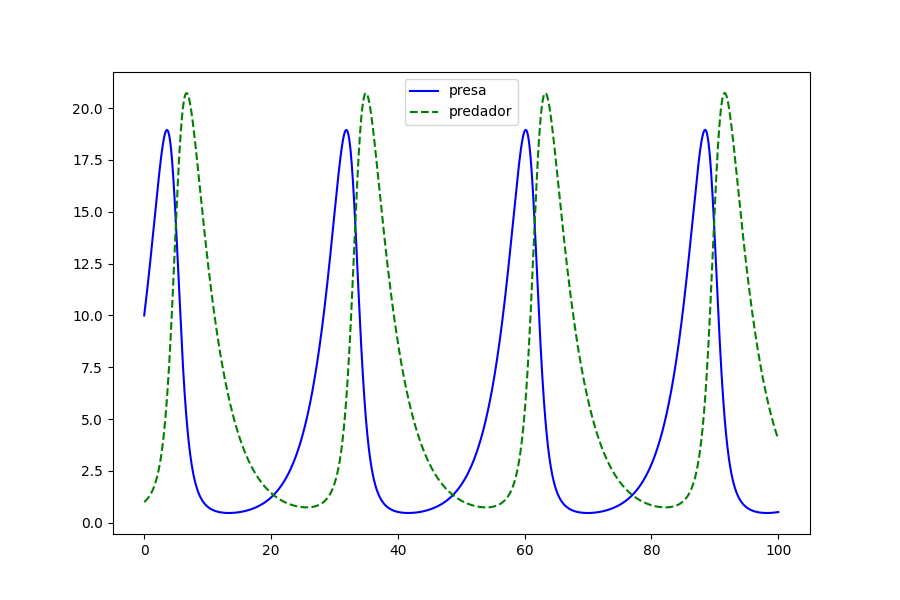
\includegraphics[scale=0.6]{imgs/hostprey.png} 
    \caption{Exemplo de resultado do modelo Predador-Presa clássico.}
    \label{fig:hostprey}
\end{figure}


%\subsection{Modelo da competição entre espécies}

%\subsection{Modelo SIR de transmissão de doenças}

\section{Programação Visual e Editores baseados em Nós}
\label{sec:programacao-visual}

Programação visual é uma maneira do usuário programar a máquina por meio de elementos gráficos que abstraem instruções do computador. Comumente, estes elementos representam múltiplas operações por vez, com o objetivo de facilitar a programação.

Um dos primeiros exemplos da aplicação prática da programação visual foi com a linguagem GRAIL (\textit{GRAphical Input Language}) \cite{grail}, desenvolvida em 1969 junto a um dispositivo semelhante a uma caneta e uma tela sensível ao seu toque. O conjunto do \textit{hardware} e do \textit{software} permitia que o usuário desenhasse letras e formas geométricas que se traduziriam em elementos de fluxograma. O objetivo era realizar um estudo sobre a comunicação humano-computador.

O conceito de utilizar elementos visuais para a assistência da programação não se restringiu somente a dispositivos especializados, contudo, e hoje se encontra em diversos \textit{softwares} de finalidades distintas que podem ser instalados em qualquer computador. Como um exemplo de aplicação de propósito similar ao GRAIL, a linguagem Scratch \cite{scratchlang} foi criada com o objetivo de facilitar o ensino de lógica de programação para crianças sem comprometer em funcionalidades. A linguagem apresenta comandos, funções e estruturas de controle como blocos que podem ser ``montados'' para compor um programa.

Outras aplicações se especializam em algum nicho da computação, como é o caso do simulador lógico Logisim \cite{logisim}, que abstrai componentes lógicos e permite o usuário criar circuitos em uma espécie de \textit{protoboard} digital.

Muitas vezes, \textit{softwares} que incluem programação visual para a abstração de operações utilizam uma interface conhecida como editor de nós:

\begin{itemize}
    \item O \textit{software} de modelagem, animação e edição de vídeos, Blender \cite{blender}, utiliza um editor de nós para abstrair operações de manipulação de imagens e materiais;

    \item O motor de jogos proprietário Unreal Engine\footnote{\href{https://www.unrealengine.com/}{Documentação da Unreal Engine}} utiliza editores de nós para múltiplas finalidades e, entre elas, está a escrita de \textit{shaders} e a programação de lógica geral dos jogos.
\end{itemize}

Existem diversos motivos pelos os quais a programação visual se encontra em tão amplo uso. Principalmente, pode-se atribuir o sucesso de sua aplicação à facilidade de utilização. Em geral, não se faz necessário a leitura de manuais da mesma forma que se faz com linguagens de programação tradicionais; todas as operações possíveis no software estão modeladas como elementos visuais com parâmetros de entrada e saída bem definidos. Implementações exemplares também proibirão o usuário de realizar ligações inválidas diretamente na interface, realizando uma etapa mais comum em compiladores ou analizadores estáticos de código, que geralmente permitem que o usuário cometa um ou mais erros e só descubra-os posteriormente.

\section{Geração de código}

A fase de geração de código geralmente é a última fase da compilação. Na maioria dos compiladores, o gerador de código recebe como entrada uma ou mais representações intermediárias do código/texto de entrada e retorna como saída o código/texto na linguagem alvo \cite{dragonBook}. 

Como este trabalho tem o objetivo de possibilitar a geração de código em múltiplas linguagens alvo diferentes, surgiu a necessidade de abstrair mais esta fase, de forma que a implementação de linguagens alvo adicionais seja mais simples dado que ao menos uma já foi implementada.

Para tal abstração, seguiu-se um padrão utilizado por diversos compiladores diferentes, que consiste na separação do \textit{back-end} (que trabalha com a linguagem alvo) do \textit{front-end} (que trabalha com a linguagem fonte) através da utilização de uma ou mais representações intermediárias. 

Nas próximas subseções, serão apresentados alguns conceitos importantes para o entendimento do processo de geração de código. 

\subsection{Representação intermediária}

As representações intermediárias (RIs) são usadas em um compilador por várias razões \cite{dragonBook}, dentre as quais destaca-se: 
\begin{itemize}
    \item Separar o \textit{front-end} do \textit{back-end}. Neste caso, o \textit{front-end} não precisa se preocupar com detalhes da linguagem alvo e o \textit{back-end} não precisa conhecer detalhes da linguagem fonte;
    \item Permitir que sejam realizadas otimizações independente de máquina ou otimizações independente da linguagem alvo; 
    \item Para facilitar a tradução e geração do código alvo.    
\end{itemize}

Algumas RIs usadas em compiladores incluem:  
\begin{itemize}
    \item Árvore de Sintaxe Abstrata (ASA); 
    \item Grafos Acíclicos Dirigidos (GAD); 
    \item Código de Três Endereços. 
\end{itemize}

As Árvores de Sintaxe Abstratas são muito usadas na representação do código fonte de entrada, representando comandos e expressões em cada escopo. As Árvores de Sintaxe Abstratas geralmente são utilizadas para realizar diversas verificações semânticas no código e elas podem ser a entrada para o algoritmo que gera uma outra RI mais próxima da linguagem alvo como, por exemplo, o Código de Três Endereços. O Código de Três Endereços é uma representação que está próxima da linguagem Assembly e pode ser usada como base para várias otimizações independentes de máquina. Geralmente, o Código de Três Endereços otimizado é a entrada recebida pelo gerador de código Assembly. O Código de Três Endereços também pode ser utilizado pelo algoritmo de alocação de registradores como uma abstração inicial para a escolha e atribuição de registradores. Os Grafos Acíclicos Dirigidos são muito usados para realizar algumas otimizações no código como, por exemplo, verificação de variável morta, propagação de constantes e cópias, entre outras otimizações. 

%TODO: Falar da representação intermediária do LLVM e a sua importância no desenvolvimento de compiladores que utilizam o back-end do LLVM para gerar código para várias arquiteturas. 

Como uma alternativa mais abstrata ao Assembly (que é dependente da arquitetura alvo), existe a linguagem intermediária da LLVM (LLVM \textit{Intermediate Representation}), que pode ser transpilada para o Assembly da máquina alvo. A LLVM é uma infraestrutura para o desenvolvimento de compiladores com o objetivo de facilitar o desenvolvimento de compiladores abstraindo toda a parte do backend. O desenvolvedor não precisa se preocupar em conhecer e programar para as arquiteturas alvo com as quais quer trabalhar porque, considerando que a linguagem criada possa ser transpilada na representação intermediária da LLVM (LLVM IR), ela pode ser compilada em qualquer arquitetura suportada pela infraestrutura que incluem, mas não estão limitadas a, x86, AMD64, ARM, ARM64, WebAssembly\footnote{\href{https://webassembly.org/}{WebAssembly Website}} e RISC-V.

Para facilitar o processo de geração de código e realizar uma maior separação entre o \textit{front-end} (interface gráfica) e o \textit{back-end} (gerador de código) do software, foi criada e utilizada uma representação intermediária (RI). A RI é a entrada para o gerador de código e também é utilizada para salvar e carregar os modelos construídos no software. A RI desenvolvida será apresentada e explicada na Seção \ref{subsection:RI}.

\subsection{Sistemas baseados em \textit{templates}}
 
Em várias aplicações, a geração de código é feita com base em \textit{templates}. Desde o início da \textit{World Wide Web}, \textit{templates} têm sido usados por \textit{frameworks} para ajudar no processo de construção de páginas Web. Informalmente, podemos dizer que um \textit{template} é um esqueleto (uma estrutura) que serve de referência para todo o processo de geração de código.

Em sua essência, \textit{templates} são arquivos com marcadores especiais que podem ser substituídos por outros valores dinamicamente, de forma similar ao pré-processador de C. Adicionalmente, alguns motores de \textit{templates} introduzem estruturas de controle de fluxo, como condicionais, laços de repetição e chamadas de funções para facilitar a injeção de código nos \textit{templates}.  

Para ilustrar a ideia, suponha o \textit{template} abaixo criado com base em um código que implementa um sistema de Equações Diferenciais Ordinárias (EDOs):  

\begin{lstlisting}[language=Python, firstnumber=1]
from scipy.integrate import solve_ivp
import numpy as np
import pandas as pd

def odeSystem(t, P,  {{key}}  {{key}}, ):
## for key, value in vars
    {{key}} = P[{{loop.index}}]
## endfor
## for key, value in odes
    d{{key}}_dt = {{value}}
## endfor     
    return  [ d{{key}}_dt  d{{key}}_dt, ]
\end{lstlisting}

O \textit{template} acima utiliza os marcadores definidos pela biblioteca Inja\footnote{\href{https://github.com/pantor/inja}{https://github.com/pantor/inja}}, e demonstra algumas das estruturas de controle mencionadas, na forma das palavras-chave \texttt{\textcolor{codepurple}{for}}, \texttt{\textcolor{codepurple}{if}} e \texttt{\textcolor{codepurple}{else}}.

%\section{Simulação computacional}

%Chama-se de simulação computacional o processo dinâmico de instanciar um modelo, seja este tradicional (expressado por equações) ou mais abstrato (expressado por objetos, agentes, operadores ou algoritmos), como definido em \cite{compsim}. 

%Estas simulações possibilitam a existência diversos serviços que hoje são essenciais para os seres humanos, como previsão do tempo (), construção de aviões aero-dinâmicos () e estudos de epidemias ().

%As simulações computacionais também permitem a avaliação de diferentes cenários em pouco tempo. Para as EDOs, isto possibilita a compreensão do efeito que cada componente tem no resultado final.

% Simulação computacional: 
% 	- O que é?
% 	- Qual a sua importância?
% Simulação de cenários: 
% 	Uma abordagem baseada em cenários se mostra interessante porque através desses diferentes cenários é possível compreender melhor como cada célula/substância do modelo interage e como os comportamentos emergem a partir dessas interações. Outra característica importante é a possibilidade de se analisar os efeitos de remover determinada célula/substância do modelo. 

\section{Ensino-aprendizagem de Modelagem Computacional} %TODO

%Falar sobre Metodologias ativas, aprendizagem baseada em problemas/projetos (Problem based learning) 

Os modelos são abstrações do mundo real. Com a evolução dos computadores e o seu uso massivo, os modelos computacionais têm contribuído significativamente para o avanço do conhecimento em diversas áreas. Eles nos ajudam a compreender os fenômenos de interesse permitindo “rastrear” e entender as mudanças que estão ocorrendo em um sistema complexo e visualizar, por exemplo, o efeito de uma pequena mudança no restante do sistema. 

Simulações computacionais são ferramentas fundamentais não só para a pesquisa científica, mas também para a educação. Elas são frequentemente usadas como laboratórios virtuais para promover a compreensão dos alunos sobre os conceitos teóricos que estão na base dos sistemas simulados. [Imagining the School of the Future Through Computational Simulations: Scenarios’ Sustainability and Agency as Keywords]. 

Após a Segunda Guerra Mundial, o leque de campos disciplinares em que as simulações começaram a ser utilizadas tem vindo a expandir-se até os dias de hoje, de modo que é quase impossível nomear qualquer disciplina que não tenha utilizado ou desenvolvido ferramentas computacionais e simulações para avançar a fronteira do conhecimento (Borrelli e Wellmann, 2019).

O uso de modelos computacionais abre novas maneiras para os alunos aprenderem sobre diferentes disciplinas. Os alunos podem aprender através de um processo iterativo de construção do modelo, simulação, modificação do modelo para simulação novamente, explorando todas as características do modelo em si [Imagining the School of the Future Through Computational Simulations: Scenarios’ Sustainability and Agency as Keywords]. Plataformas como, por exemplo, a Netlogo [ref] permitem este tipo de aprendizagem iterativa e interativa.

Um dos objetivos do software que foi desenvolvido neste trabalho é auxiliar o aprendizado de conceitos importantes nas áreas de modelagem matemática e computacional e ajudar o aluno a desenvolver a habilidade de modelar problemas através da prática de construção e simulação de modelos. O uso combinado do software com alguma metodologia ativa de ensino permitirá aos alunos aprender na prática como construir modelos para diferentes fenômenos de interesse e entender melhor os fenômenos estudados através das simulações computacionais realizadas de forma interativa através da interface gráfica do software. 

Considerando o uso do software na prática e uma visão geral do chamado ciclo da modelagem apresentado na Figura \ref{fig:ciclo-modelagem}, destaca-se que o software auxilia o passo 2 e automatiza os passos 3 e 4 facilitando o processo de modelagem por estudantes e pesquisadores. 

\begin{figure}[h]
    \centering
    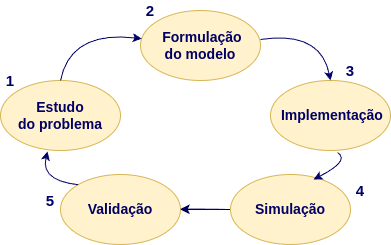
\includegraphics[scale=0.5]{imgs/ciclo-modelagem.png} 
    \caption{Visão geral do ciclo da modelagem.}
    \label{fig:ciclo-modelagem}
\end{figure}

O aprendizado, em sala de aula, pode ser conduzido, por exemplo, através de um processo incremental que começa investigando e trabalhando com modelos mais simples até se chegar em modelos mais complexos. Algumas vantagens dessa abordagem incluem:  1) a apresentação de determinados conceitos e técnicas é facilitada em modelos mais simples; 2) em muitos casos reais, modelos complexos utilizam certas expressões, equações e “estratégias” na modelagem que estão presentes em modelos mais simples. Então, muitas vezes, o aluno conseguirá entender melhor um modelo mais complexo entendendo que determinadas partes do mesmo já apareceram em modelos mais simples previamente estudados. 

Uma possível abordagem de ensino seria o professor trabalhar com algum problema escolhido por ele para apresentar e discutir conceitos e/ou técnicas de modelagem de forma semelhante à metodologia \textit{Problem Based Learning} (PBL) [refs]. O seguinte conjunto de passos é sugerido para o processo de estudo, modelagem e simulação computacional: 

\begin{enumerate}
 \item Descrição do contexto e do problema a ser modelado;
 \item Formulação das hipóteses pelos alunos e discussão entre eles;
 \item Formulação do modelo considerando o conhecimento de modelos existentes e que foram estudados previamente;
 \item Construção do modelo no software;
 \item Simulação do modelo no software com a criação de diferentes cenários para teste e análise dos comportamentos obtidos.
 \item Avaliação dos resultados do modelo com a ajuda do professor: caso o comportamento desejado ou esperado não seja obtido, voltar para um dos passos anteriores como, por exemplo, o passo 2 ou 3 e repetir o processo. 
\end{enumerate}

A ideia dessa abordagem é colocar o aluno como protagonista no processo de construção do próprio conhecimento porque o aluno estará ativamente realizando todas as etapas de modelagem do problema. O software irá facilitar a construção e simulação do modelo de forma que os alunos poderão gastar mais tempo formulando as hipóteses e equações do modelo, planejando os cenários a serem simulados e avaliando os resultados obtidos. 

%---------------------------------//-----------------------------
\chapter{Trabalhos relacionados}
\label{chap:relacionados}

Com o avanço de tecnologias para o desenvolvimento de aplicações gráficas e também da internet, ocorreu um aumento expressivo na quantidade de \textit{softwares} desenvolvidos para modelagem e simulação computacional. 

Na Tabela \ref{tab:comparativo} é apresentado um quadro comparativo entre o software deste trabalho e softwares similares. Para realizar a comparação, foram selecionadas algumas características consideradas relevantes no contexto de softwares para modelagem e simulação computacional. 

\begin{landscape}
\begin{table}[h]
    \centering
        \begin{tabular}{m{0.2\textwidth}m{0.25\textwidth}m{0.3\textwidth}m{0.2\textwidth}m{0.15\textwidth}m{0.15\textwidth}m{0.15\textwidth}}
        \toprule
        \multicolumn{1}{c}{} & \multicolumn{1}{c}{} & \multicolumn{2}{c}{\textbf{Acesso}} & \multicolumn{3}{c}{\textbf{Funcionalidades}} \\
        \cmidrule(rl){3-4}\cmidrule(rl){5-7}
        \textbf{Software} & {Modelos} & {Distribuição} & {Open Source?} & {Representação Gráfica?} & {Exporta Código?} & {Simulação Interativa?} \\
        \midrule
        ODE Designer & EDOs & Desktop com dependências inclusas & Sim & Sim & Sim & Sim \\
        Snoopy & Redes de Petri & Desktop com dependências inclusas & Não & Sim & Não & Sim \\
        VCell & EDOs, EDPs e modelos Estocásticos & Desktop com dependências inclusas & Sim & Sim** & Não & Sim \\
        InsightMaker & EDOs, Dinâmicas de Sistemas, Modelos baseados em Agentes & Aplicação Web & Não* & Sim** & Não & Sim \\
        Cytoscape & Redes Complexas & Desktop & Sim & Sim & Não & Sim \\
        EpiFire & Redes de Contatos (\textit{Contact Networks}) & Desktop com dependências inclusas & Sim & Não & Não & Sim \\
        \bottomrule
    \end{tabular}
    \caption{Tabela comparativa entre os principais softwares de modelagem computacional e o software desenvolvido neste trabalho. \\ *Apenas a biblioteca de simulação é \textit{open source}, não incluindo a interface gráfica. \\ **Os modelos são escritos em formas de equações e não necessariamente serão representados fielmente pela representação gráfica destes softwares.}
    \label{tab:comparativo}
\end{table}
\end{landscape}

O software desenvolvido neste trabalho possui alguns diferenciais em relação a outros desenvolvidos com propósitos similares:

\begin{itemize}
    \item Em sua interface gráfica, é apresentado um editor baseado em nós que fornece ao usuário uma forma de programação visual \ref{sec:programacao-visual} que facilita a construção e simulação de modelos, limitando apenas operações consideradas incorretas;
    %possibilitando um grau de liberdade limitando apenas operações consideradas incorretas;
    
    \item Em seu formato de representação intermediária para salvamento e carregamento dos modelos, o software utiliza uma estrutura extensível para outros tipos de modelos como, por exemplo, equações diferenciais parciais. Esta estrutura também foi projetada para ser humanamente legível, a ponto de ser possível que uma pessoa decodifique o modelo representado apenas lendo o arquivo. Assim, caso o software se prove insuficiente ou indisponível, ainda é possível reverter o arquivo nas equações que o compõe. 
    
    \item O software permite ao usuário acessar o código-fonte usado para simular o modelo, possibilitando que o usuário conheça o código usado na simulação e também possa utilizar e alterar o código como desejar.   
\end{itemize}

Poucos \textit{softwares} encontrados na literatura permitem que o usuário visualize e interaja com o código gerado para a simulação de seu modelo. Mais comumente, a única maneira com a qual o usuário pode interagir com o modelo é através da abstração provida pela interface, o que causa uma dependência direta do \textit{software}.

A seguir, são descritos em mais detalhes os trabalhos relacionados. 

\section{Snoopy}

Um \textit{software} que serviu como inspiração para este trabalho foi o software para construção, animação e simulação de redes de Petri chamado Snoopy \cite{Heiner2008,Heiner2012,Liu2012}. Além da rede de Petri clássica, o software permite modelar e simular vários tipos de redes de Petri como, por exemplo, redes de Petri estocásticas e coloridas que são extensões da rede clássica. O modelo construído é representado como um grafo que tem dois tipos de nós chamados \textit{places} (locais) e \textit{transitions} (transições) e quatro tipos de arestas (estocástica, imediata, determinística e planejada) com suas semânticas associadas. Os \textit{places} representam populações de um certo tipo e transições representam eventos que podem aumentar ou diminuir as quantidades das populações que estão armazenadas nos locais. 

O modelo gráfico utilizado pelo software Snoopy serviu de inspiração para a criação da representação visual utilizada neste trabalho. A partir do software Snoopy, foi possível observar que modelos gráficos, além do atrativo visual, facilitam a construção do modelo, e um melhor entendimento do que está sendo feito e o que está sendo modelado. A possibilidade de simular interativamente as Redes de Petri estocásticas foi um fato que serviu de inspiração para a ideia da simulação interativa no software desenvolvido neste trabalho. 

\section{Insight maker}
    
O InsightMaker \cite{insightmaker} é um \textit{software} de simulação baseado em nuvem. Todo o modelo é feito através de um navegador de internet e, quando executado, é simulado no próprio servidor, sem a necessidade de que o usuário possua uma máquina potente. O InsightMaker \cite{insightmaker} permite a construção de modelos utilizando diagramas de Dinâmica de Sistemas e modelos baseados em agentes. O site possui diversos recursos para a construção do modelo em um Canvas. A partir do modelo de Dinâmica de Sistemas construído no Canvas, o InsightMaker \cite{insightmaker} gera internamente um modelo de EDOs e executa este modelo utilizando o método de Euler ou o método de Runge-Kutta de quarta ordem conforme escolha do usuário. Através da interface web, também é possível definir os valores de todas as variáveis e parâmetros, e é possível realizar as simulações computacionais. Os resultados são exibidos de forma interativa onde é possível controlar a velocidade com que os valores são exibidos nos gráficos. 

\section{VCell}

O software VCell (Virtual Cell) \cite{vcell,VCellref1} é uma plataforma para modelar sistemas biológicos celulares que é construída em torno de um banco de dados central e disseminada como um aplicativo da web. Os modelos são construídos com base em regras (\textit{Rule-based modelling}). VCell tem os seguintes tipos de simulações disponíveis: determinística (EDO compartimental ou EDP de reação-difusão-advecção com suporte para cinemática 2D), reações estocásticas (solvers de SSA), estocástica espacial (reação-difusão com Smoldyn), híbrida determinística/estocástica e simulações baseadas em agentes. O software permite simular vários processos metabólicos que ocorre dentro das células e através das membranas celulares. Com relação às membranas, há suporte para os seguintes processos: Eletrofisiologia, suporte para o fluxo da membrana e difusão lateral da membrana. 

Durante alguns testes com o VCell \cite{vcell,VCellref1}, sentiu-se a necessidade da leitura de um manual dado o fato de que o software apresenta muitas opções nas diferentes telas que são abertas para a construção de um modelo de EDOs. Durante os testes, não foi possível entender como o modelo de EDOs é construído e qual é o sistema de equações final que é usado na simulação. Acredita-se que isso tenha ocorrido devido ao software apresentar muitas telas com muitas opções diferentes o que torna difícil entender e navegar pelas diferentes opções. 

\section{EpiFire}

O EpiFire \cite{epifire} não é um \textit{software} completo, mas uma biblioteca em C++ para simulação de modelos de redes complexas com aplicação na área de Epidemiologia. Ele é uma interface de programação de aplicativos (API) implementado em C++, projetado para gerar de forma eficiente redes com uma distribuição de grau especificada, medir características fundamentais da rede e realizar simulações computacionais eficientes das redes geradas com base nos métodos \textit{percolation} e \textit{chain-binomial}. 

\section{Cytoscape}

O software Cytoscape \cite{shannon2003cytoscape} é uma plataforma de software de código aberto para visualizar redes de interação molecular e vias biológicas e integrar essas redes com anotações, perfis de expressão gênica e outros dados. O software permite carregar conjuntos de dados de interação molecular e genética em vários formatos padrão. O sistema de \textit{plugins} permite a extensão do software através de diversas aplicações desenvolvidas seguindo uma API baseada no modelo OSGi. O Cytoscape também é utilizado como uma plataforma geral para análise e visualização de redes complexas. 


%OpenFOAM (https://www.openfoam.com/)
%Stella (https://www.iseesystems.com/store/products/stella-online.aspx)


\chapter{Software para modelagem e simulação computacional}
\label{chap:metodologia}
\label{chap:software-para-modelagem}

O \textit{software} desenvolvido neste trabalho consiste em uma interface gráfica de usuário [\ref{fig:gui-predador-presa}] (mais comumente referida pelo acrônimo em inglês, GUI, que significa \textit{Graphical User Interface}) que apresenta um editor baseado em nós. Os nós representam abstrações de componentes comumente usados na construção de EDOs, como constantes e variáveis. Em \ref{sec:representacao-visual-edo}, serão discutidos os tipos de nós presentes na interface.

\begin{figure}[h]
    \centering
    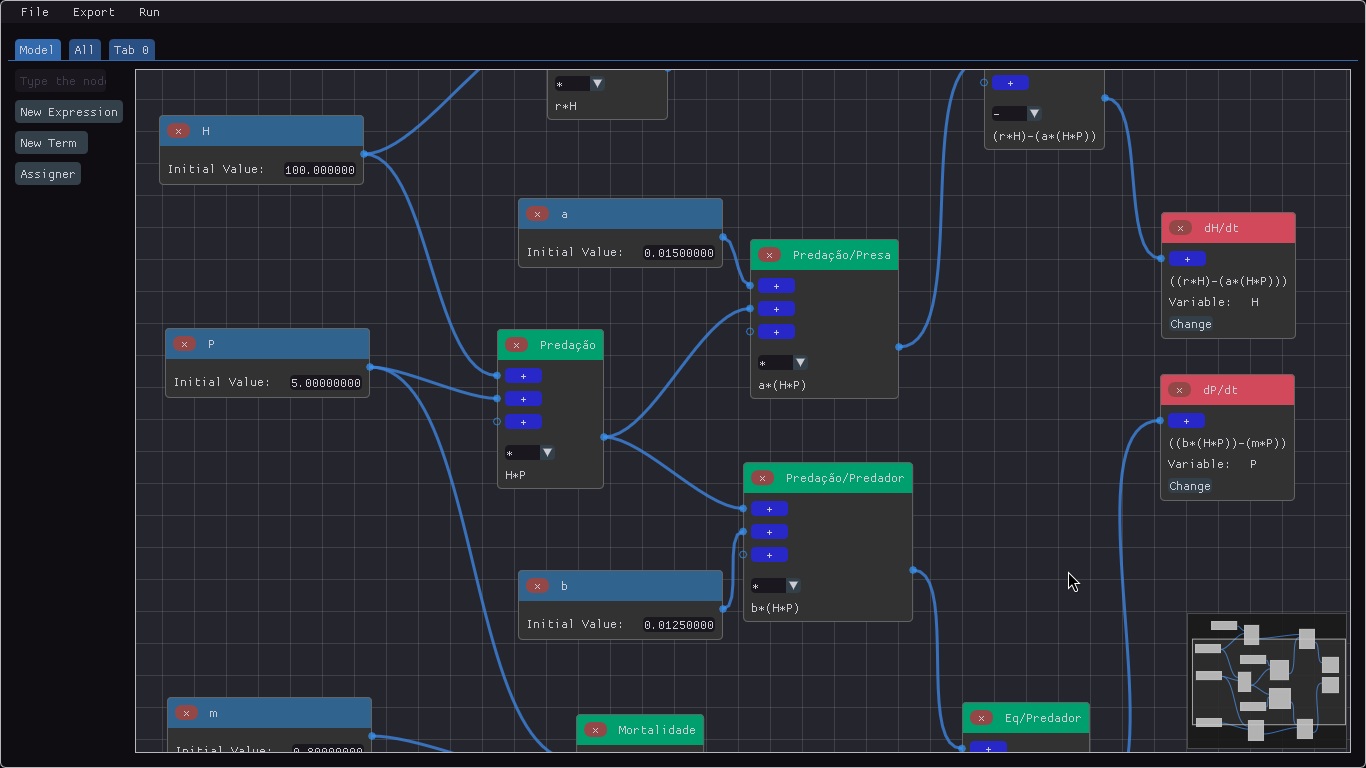
\includegraphics[scale=0.35]{imgs/ode-designer/predador-presa.png} 
    \caption{Exemplo do modelo Predador-Presa (\ref{eq:predadorpresa}) construído no \textit{software}.}
    \label{fig:gui-predador-presa}
\end{figure}

O modelo é construído a partir da criação de nós e suas ligações. Uma equação pode ser expressada por um ou mais termos e combinações, e uma variável alvo para a atribuição do valor.

Após construído o modelo, o usuário poderá simulá-lo diretamente pela GUI [\ref{fig:gui-grafico-all}], exportar um PDF dos resultados, ou exportar um código de Python equivalente para o modelo desenhado [\ref{code:predador-presa}]. A experiência de usuário pode ser resumida ao fluxograma \ref{fig::experiencia_usuario}.

\begin{figure}[h]
    \centering
    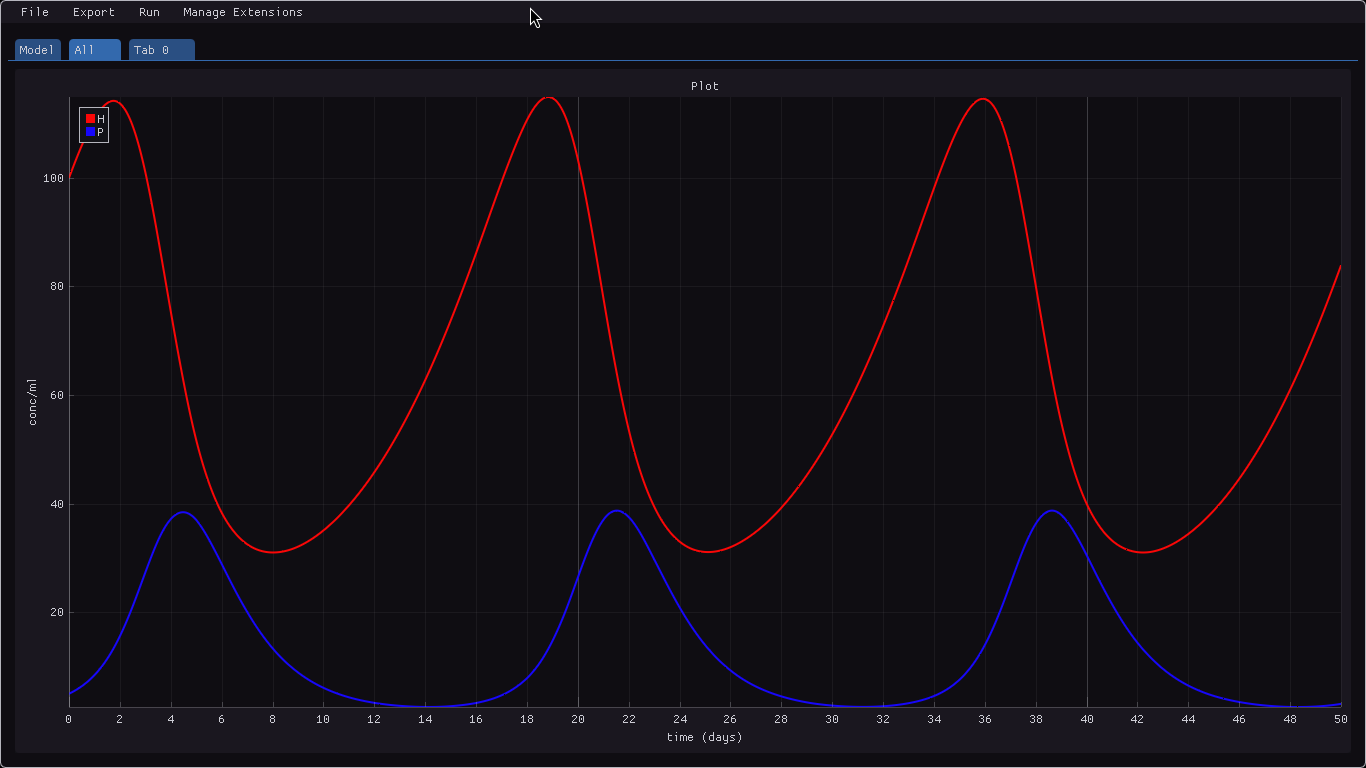
\includegraphics[scale=0.35]{imgs/ode-designer/grafico-all.png} 
    \caption{Plotagem dos resultados da simulação do modelo Predador-Presa.}
    \label{fig:gui-grafico-all}
\end{figure}

\begin{figure}[h]
    \centering
    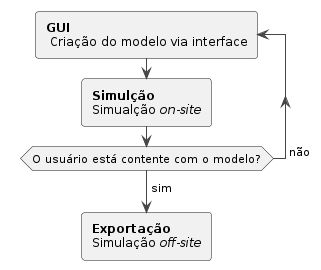
\includegraphics[scale=1]{diagrams/img/fluxograma-exp.png}
    \caption{Fluxograma da experiência de usuário esperada para o software.}
    \label{fig::experiencia_usuario}
\end{figure}

Dessa forma, o usuário pode criar e simular modelos sem a necessidade de iniciar a implementação computacional do zero e também sem a necessidade de ter conhecimentos dos métodos que são utilizados na implementação. Pelo contrário, o usuário terá acesso aos códigos gerados e poderá aprender com estes e utilizá-los, por exemplo, como base para desenvolver o seu próprio código. 

A simulação das EDOs, tanto pela GUI quanto pelo código de Python exportado, é feita utilizando métodos especializados da biblioteca ciêntífica \texttt{scipy} \cite{scipy}. % TODO: Devemos entrar em detalhes de como isso é feito? Se sim, precisamos de uma explicação do método RK45

\section{Uma representação visual para EDOs}
\label{sec:representacao-visual-edo}

Uma representação visual foi desenvolvida para minimizar a necessidade de um conhecimento técnico prévio pelo usuário, assim como a dependência de documentos e manuais. Para atingir este objetivo, foi necessário modelar esta representação utilizando conceitos que fossem naturais para o público-alvo e a forma com a qual este desenvolve EDOs.

A construção de EDOs se baseia em alguns princípios gerais, como a Lei de Ação de Massas. Por exemplo, dado duas populações $A$ e $B$, caso seja desejado simular uma condição que seja mais provável de acontecer dado altas concentrações de ambas as populações, é possível representá-la simplesmente multiplicando ambas as populações. Opcionalmente, adiciona-se uma constante para controlar a taxa de ocorrência.

No sistema de EDOs \ref{eq:predadorpresa}, é possível visualizar este fenômeno: na equação da presa, a expressão \(-a.H.P\) é utilizada para controlar a taxa de predação, isto é, o quanto a concentração desta população é afetada negativamente pela atividade de predação realizada pelos predadores. Naturalmente, a predação ocorrerá mais frequentemente dado altas concentrações de ambos presa e predador, assim como descrito acima.

A partir desta premissa, pode-se resumir o desenvolvimento de EDOs à combinação das expressões que representam as interações das populações entre si e o meio. Assim, a representação visual foi modelada em um editor de nós, de forma que todas as interações visassem a construção destas expressões. A tabela \ref{tab:tipos-de-nos} descreve os tipos de nós presentes no software e sua relação com o objetivo de construir as expressões.

\begin{table}
\begin{center}
\begin{tabular}{ |m{0.12\textwidth}|m{0.35\textwidth}|m{0.5\textwidth}| }
    \hline
    \rowcolor{lightgray} Tipo de nó & Usado para representar & Exemplo \\
    \hline
    Termo & Variáveis, parâmetros e constantes. & Em uma expressão \(k.x.y\), os termos são o parâmetro $k$ e as variáveis $x$ e $y$. \\
    \hline
    Expressão & Qualquer expressão matemática para a construção das equações do modelo. & Na equação da presa [\ref{eq:predadorpresa}], as expressões são: 1) \(r.H\); 2) \(a.H.P\); e 3) \(r.H - a.H.P\) (combinação de 1 e 2). \\
    \hline
    Equação & É um nó especial usado para atribuir uma expressão, que representa todo o lado direito de uma EDO, a uma variável. & A expressão \(r.H - a.H.P\) pode ser usada como entrada de um nó de equação associado à variável $H$. \\
    \hline 
\end{tabular}
\end{center}
\caption{Tipos de nós presentes no software.}
\label{tab:tipos-de-nos}
\end{table}

\subsection{Representação de expressões na interface}
\label{subsec:exprtree}

Na GUI, os nós de expressão apresentam a expressão que estão construindo, para que o usuário não tenha que inspecionar cada nó individiualmente para determinar como uma expressão está sendo formada. Desta forma, não é necessário observar apenas a equação final. Isto é feito por meio de árvores de expressões que cada um destes nós carrega consigo.

Na imagem \ref{fig:expr-tree} são apresentadas as árvores de expressões de todos os nós presentes em \ref{fig:gui-predador-presa}. Note que os nós `Predação/Presa' e `Predação/Predador' referenciam o mesmo nó base `Predação'. Isto demonstra expressões podem ser usadas como entradas para outras expressões na forma de subexpressões. As subexpressões, além de possibilitar o usuário de evitar repetições na construção de modelos, permitem que os nós façam alterações relevantes para o contexto, como a adição de parênteses nas operações de multiplicação e divisão.

Esta representação foi desenvolvida de maneira agnóstica ao modelo, com o objetivo de permitir que o software seja extensível e, no futuro, oferte outros tipos de modelos. Um exemplo deste esforço se dá pela árvore de expressões não supôr que toda operação é infixada, também permitindo operações pós-fixadas. Exemplos da estensibilidade serão apresentados em \ref{sec:estensibilidade}, enquanto o futuro será discutido em \ref{sec:futuro}.

\begin{figure}[h]
    \centering
    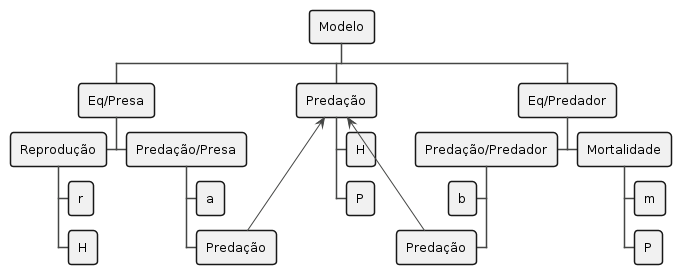
\includegraphics[scale=0.65]{diagrams/img/expr-tree.png} 
    \caption{Árvores de expressões para cada nó de expressão no modelo predador-presa [\ref{fig:gui-predador-presa}]}
    \label{fig:expr-tree}
\end{figure}

\subsection{Uma representação intermediária humanamente legível}
\label{subsection:RI}

Com a finalidade de possibilitar a escrita e leitura em disco dos modelos desenhados na GUI, uma RI foi definida. O formato JSON foi escolhido por sua popularização com a \textit{web} e com sua clara representação de estruturas de dados como listas e tabelas \textit{hash} que facilitam o desenvolvimento do software. A escolha de um formato pré-estabelecido também torna a RI mais resiliente a futuras mudanças, uma vez que não será necessário modificar a sintaxe do formato e nem as bibliotecas que o interpretam.

Apesar de ser usada como forma de armazenar informações do modelo, a RI possui um formato projetado para ser humanamente legível. Esta decisão foi tomada para possibilitar a recuperação do modelo construído sem a necessidade de ter o software instalado. Assim, caso o software caia em desuso, se torne impossível de instalar por algum motivo (um sistema operacional diferente, por exemplo) ou simplesmente tenha mudanças que quebrem compatibilidade implementadas, não significa que o usuário tenha perdido seu 
modelo.

Em \ref{ri:presa}, pode-se observar o trecho da RI do modelo Predador-Presa [\ref{ri:predador-presa}] que implementa a equação da presa. Note que é possível reconstruir a equação manualmente: cada entrada em \texttt{"arguments"} representa um termo (representado pelos campos nome e valor) ou uma combinação (representada pelos campos nome, operação e composição). Com este último, uma expressão pode ser construída a partir da repetida concatenação de todos os elementos de sua composição, inserindo a operação entre eles. Seguindo esta regra, tem-se as seguintes expressões:

\begin{itemize}
    \item \texttt{"Predacao/Presa"}: \((+a)*(+H)*(+P)\), que simplificando se resume a \(a*H*P\);
    \item \texttt{"Reprodução"}: \((+r)*(+H)\), que simplificando se resume a \(r*H\);
    \item \texttt{"Eq/Presa"}: A subtração de \texttt{"Predacao/Presa"} e \texttt{"Reprodução"}, que resulta em \(r*H-a*H*P\);
\end{itemize}

\begin{lstlisting}[language=json, label=ri:presa, caption=Trecho da RI que define termos e combinações usadas para definir a equação da presa.][H]
"arguments": [
    { "name": "Eq/Presa", "operation": "-",
        "composition": [
        { "name": "Reproducao", "contribution": "+" },
        { "name": "Predacao/Presa", "contribution": "+" }
    ]},
    { "name": "Reproducao", "operation": "*",
        "composition": [
        { "name": "r", "contribution": "+" },
        { "name": "H", "contribution": "+" }
    ]},
    { "name": "Predacao/Presa", "operation": "*",
        "composition": [
        { "name": "a", "contribution": "+" },
        { "name": "H", "contribution": "+" },
        { "name": "P", "contribution": "+" }
    ]},
    { "name": "H", "value": 100.0 },
    { "name": "P", "value": 5.0 },
    { "name": "r", "value": 0.2 },
    { "name": "a", "value": 0.015 }
]
\end{lstlisting}

\section{Geração de Código e Simulação interativa}

Além de apresentar uma interface capaz de criar, salvar e carregar sistemas de EDOs, o software também possibilita ao usuário simular o modelo (plotando os resultados na interface), gerar o código equivalente em Python ou exportar um PDF com os resultados.

A geração de código é feita por meio da injeção de informações do modelo em marcações presentes no \textit{template} e se baseia na substituição de \textit{strings}. Os \textit{templates} incluem o código base necessário para a resolução numérica, simulação e plotagem dos resultados com a inclusão de todas as bibliotecas necessárias. Os templates são escritos de maneira sucinta e legível com o objetivo de servir como um material de aprendizagem estensível.

Na listagem de código \ref{code:jinja-template}, observa-se parte do template que extrai o valor de variáveis e constantes para serem usados na simulação do próximo passo de tempo. Neste trecho, nota-se o uso de estruturas de controle como condicionais (\texttt{if}) e laços de repetição (\texttt{for}). Baseando a geração de código no sistema de \textit{templates}, é possível adicionar novas formas de simulações sem alterar o código do programa. Por exemplo, é possível adicionar um \textit{template} para gerar o código que simulará o modelo de forma estocástica usando o algoritmo de Gillespie.

\begin{lstlisting}[language=Python, label=code:jinja-template, caption=Trecho do \textit{template} responsável por extrair o valor de variáveis e constantes][H]
def system(t: np.float64, y: np.ndarray, *constants) -> np.ndarray:
    
    {{- arg.name }},
     = y

    
    
    {{- arg.name }},
     = constants
    
    # ...
\end{lstlisting}

O código gerado, além de ser aprensentado como opção de exportação do modelo para o usuário, também é utilizado internamente pelo software para produzir os resultados que são plotados na interface. Como benefício desta abordagem, os gráficos plotados tanto pelo software quanto pelo código exportado são idênticos. Por outro lado, a dependência de Python para a simulação traz complicações quanto à distribuição do software, que será discutida em mais detalhes em \ref{sec:distribuicao}, assim como será discutida a solução implementada.

\section{Estensibilidade}
\label{sec:estensibilidade}

É improvável que seja possível construir um software que atenda todas as necessidades de um público-alvo, e o software desenvolvido neste trabalho não é exceção; seria difícil determinar quais são as funcionalidades mínimas necessárias para construir qualquer sistema de EDOs. Visando, então, maximizar os casos de uso aos quais este software atende, foi desenvolvido um sistema de extensões de usuário. 

Além de prover os nós padrões [\ref{tab:tipos-de-nos}] para a construção das EDOs exemplificadas, o software permite que o usuário desenvolva e utilize extensões para realizar operações que não estão prontamente disponíveis pela interface. Estas extensões são desenvolvidas em Python e incluem funções que serão interpretadas como nós na interface.

As funções decoradas por \texttt{@node} num arquivo de extensões serão interpretadas como nós. Seus nomes são usados em sua identificação na interface, e a quantidade de parâmetros que recebem determinam a quantidade de pinos de entradas. Por padrão, estes nós `customizados' construirão expressões mais próximas da representação destas funções em linguagens de programação (como \texttt{funcao(param1, param2, ...)}), porém este comportamento pode ser sobrescrito com o parâmetro \texttt{format} no decorador.

Na listagem \ref{code:ext-sin-pow}, é apresentado um exemplo de arquivo de extensões contendo um nó para calcular o seno de um parâmetro e um nó que eleva um parâmetro ao valor de outro. Este arquivo pode ser importado na interface, que possibilitará o uso dos nós como na figura \ref{fig:ext-sin-pow}.

\begin{lstlisting}[language=Python, label=code:ext-sin-pow, caption=Exemplo de definição dos nós de extensão seno e potência com código Python válido., float, xleftmargin=.35\textwidth]
import math

@node
def sin(x):
    return math.sin(x)

@node(format='$1 ^ $2')
def pow(x, y):
    return x ** y

\end{lstlisting}

\begin{figure}[h]
    \centering
    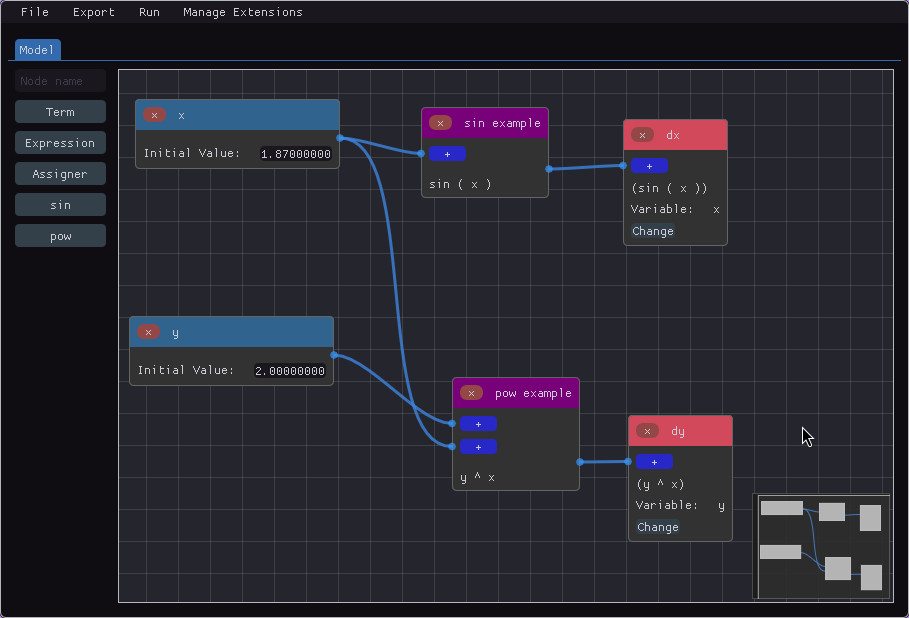
\includegraphics[scale=0.45]{imgs/ode-designer/ext-sin-pow.png} 
    \caption{Os nós definidos em \ref{code:ext-sin-pow} sendo utilizados na interface.}
    \label{fig:ext-sin-pow}
\end{figure}

Como estes nós são definidos utilizando Python, não há impacto na capacidade do software de simular o modelo e plotar os gráficos; as funções definidas nas extensões são diretamente incluídas no código final que será utilizado pela simulação. Ademais, os modelos salvos pela interface mantém uma referência aos arquivos de extensões utilizados na construção do modelo, tornando possível que o software auto-importe as extensões necessárias quando carregar um modelo do disco. Isto permite que usuários não-técnicos utilizem extensões desenvolvidas por outras pessoas.

\subsection{Carregamento de extensões}

Como mencionado anteriormente, os nós de extensões são definidos por funções que utilizam um decorador específico. Durante o carregemanto de um arquivo de extensões, o software injeta um trecho especial de código que define o decorador \texttt{@node} para inspecionar a função que está sendo decorada e emitir um JSON com as informações relevantes sobre a função como nome, quantidade e nome dos parâmetros e o formato da representação na interface. Essas informações servem como especificações para novos construtores de nós.

\section{Implementação e Tecnologias utilizadas}
\label{sec:tecnologias}

O software desenvolvido foi dividido em dois módulos: (1) o responsável pela interface gráfica e (2) o responsável pela representação intermediária. O primeiro lida com a apresentação de gráficos, interações com o usuário e a plotagem dos resultados, enquanto o segundo define a representação em JSON dos modelos e realiza a transformação em código Python.

\subsection{O módulo da GUI}
\label{sub:gui}

O módulo da GUI, desenvolvido em Rust, é a aplicação principal, e é responsável por toda a jornada do usuário. Este módulo inclui o editor de nós, o plotador de gráficos e as operações que envolvem a invocação do módulo da RI e a apresentação dos resultados destas chamadas.

Entre seus submódulos principais, estão:

\begin{itemize}
    \item O submódulo da aplicação, que renderiza o editor de nós e gerencia o estado global. A aplicação também controla as janelas auxiliares que podem ser abertas, como as abas de plotagem de resultados, o gerenciador de extensões e o atribuidor de variáveis. A figura \ref{fig:uml-app} contém o diagrama de classes desse módulo;
    \begin{figure}[h]
        \centering
        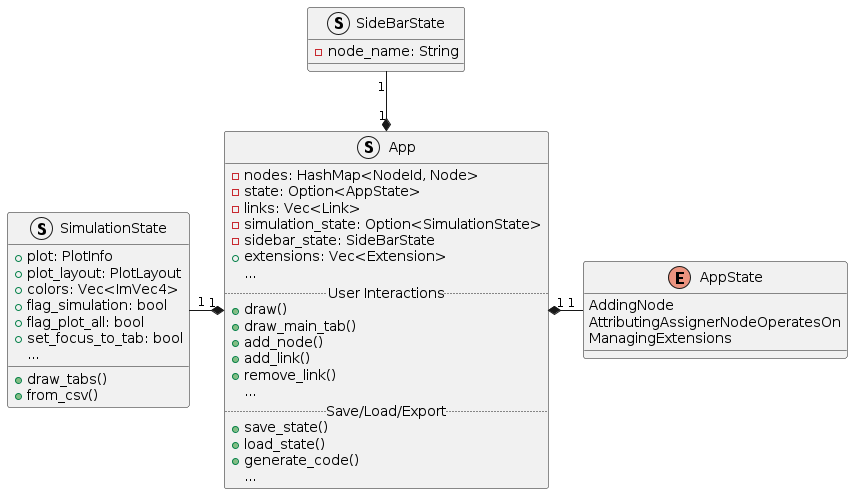
\includegraphics[scale=0.5]{diagrams/img/app.png} 
        \caption{Diagrama de classes do módulo da aplicação.}
        \label{fig:uml-app}
    \end{figure}
    \item O submódulo de nós, que define os possíveis tipos de nós. Estes possuem métodos para receber e enviar mensagens (notificando mudanças de estados, como alteração na árvore de expressão) e definir suas cores na interface. A figura \ref{fig:uml-nodes} contém o diagrama de classes desse módulo;
    \begin{figure}[h]
        \centering
        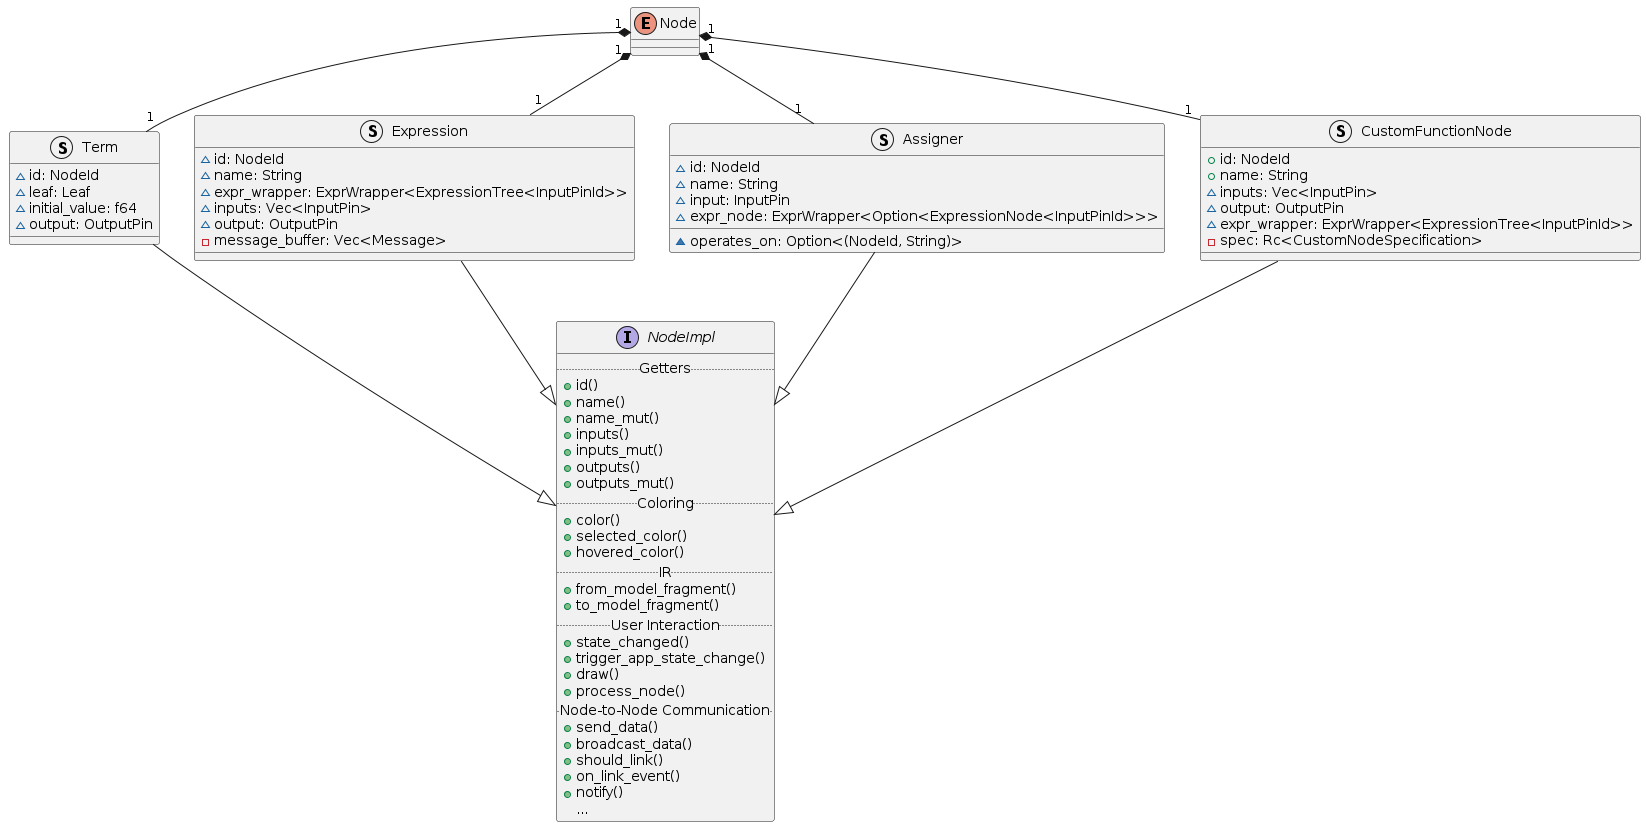
\includegraphics[scale=0.3]{diagrams/img/nodes.png} 
        \caption{Diagrama de classes do módulo de nós.}
        \label{fig:uml-nodes}
    \end{figure}
    \item O submódulo de extensão, que define as estruturas necessárias para analisar e carregar a definição de nós customizados em forma de funções de Python. A figura \ref{fig:uml-extensions} contém o diagrama de classes desse módulo;
    \begin{figure}[h]
        \centering
        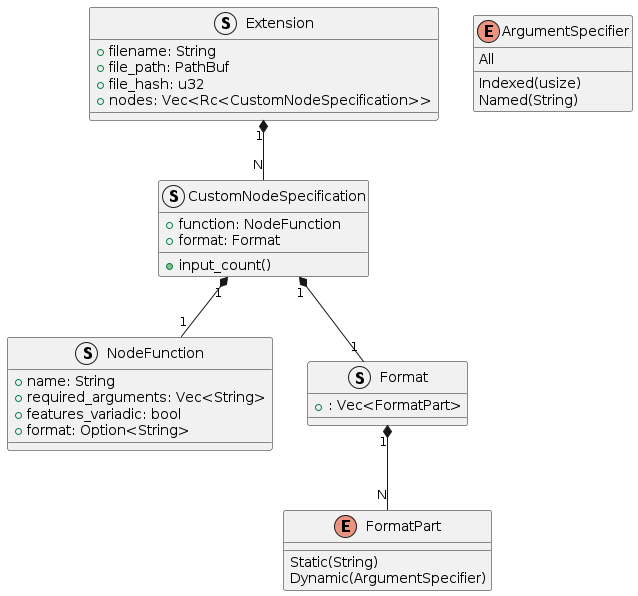
\includegraphics[scale=0.45]{diagrams/img/extensions.png} 
        \caption{Diagrama de classes do módulo de extensões.}
        \label{fig:uml-extensions}
    \end{figure}
    \item O submódulo de expressão, que define a árvore de expressões que representa o modelo e as estruturas que podem ser usadas durante a passagem de mensagens para comunicar mudanças parciais. A figura \ref{fig:uml-expr} contém o diagrama de classes desse módulo;
    \begin{figure}[h]
        \centering
        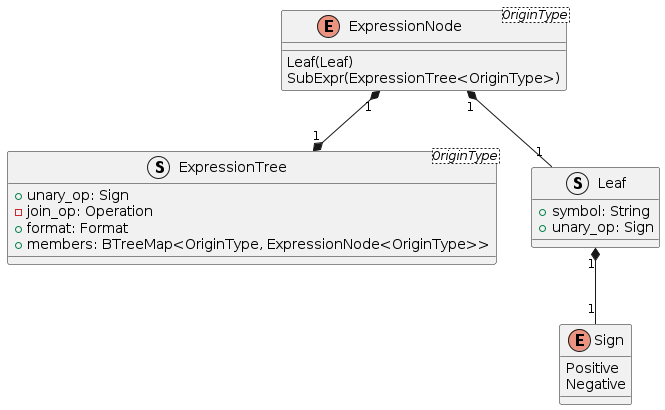
\includegraphics[scale=0.6]{diagrams/img/exprtree.png} 
        \caption{Diagrama de classes do módulo da árvor de expressões.}
        \label{fig:uml-expr}
    \end{figure}
    \item O submódulo de mensagens, que implementa a estrutura utilizada pelos outros módulos durante a comunicação intra-aplicação. A figura \ref{fig:uml-msg} contém o diagrama de classes desse módulo.
    \begin{figure}[h]
        \centering
        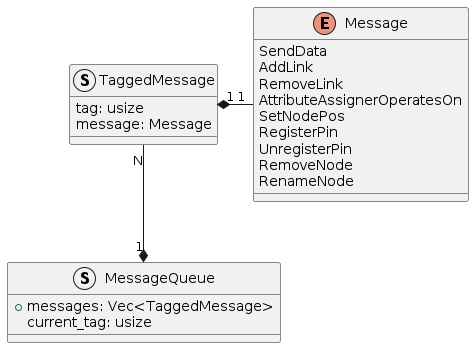
\includegraphics[scale=0.45]{diagrams/img/messages.png} 
        \caption{Diagrama de classes do módulo de mensagens.}
        \label{fig:uml-msg}
    \end{figure}
\end{itemize}

\subsection{A utilização de Rust para a GUI}
\label{sub:cpp-rust}

O módulo de GUI [\ref{sub:gui}] foi inicialmente desenvolvido em C++ e depois todo o código do software foi migrado para Rust\footnote{\url{https://www.rust-lang.org/}}. Um dos motivos foi o fato de que rapidamente se tornou desafiador manter uma grande base de código livre de \textit{bugs} relacionados a ponteiros nulos e liberações duplas (\textit{double frees}). Isto acontece porque muitas operações em C e C++ podem gerar erros que podem ser ignorados, sem que uma ferramenta de análise estática de código consiga auxiliar nestes casos. Ademais, mesmo os recursos mais recentes de segurança de memória adicionados em C++ não podem ser completamente utilizados, uma vez que não possuem uma ABI (\textit{Application Binary Interface}) estável e, portanto, não podem ser utilizados intercambiavelmente entre C++ e Rust.

A importância de evitar \textit{bugs} relacionados à segurança de memória foi ressaltada pela agência de segurança nacional dos EUA em novembro de 2022\footnote{\href{https://media.defense.gov/2022/Nov/10/2003112742/-1/-1/0/CSI_SOFTWARE_MEMORY_SAFETY.PDF}{Software Memory Safety | U/OO/219936-22}}, que, no documento citado, recomendou o uso das chamadas linguagens seguras no uso da memória (\textit{memory safety languages}) como, por exemplo, Rust, C\#, Go, Java, Python and Swift. A segurança de memória é uma propriedade de algumas linguagens de programação que evita que os programadores introduzam certos tipos de \textit{bugs} relacionados ao uso da memória como ponteiros pendentes, ponteiros nulos, \textit{buffer overflow}, entre outros. Outro motivo para a mudança de linguagem foi a disponibilidade de bibliotecas na linguagem Rust que facilitaram bastante o trabalho de salvar e carregar a RI, e também de gerar código. 

Durante o desenvolvimento, tentou-se uma solução que combinava C++ para a interface gráfica e Rust para a geração de código e gerenciamento da representação intermediária. Porém, foram encontradas complicações na implementação da interoperabilidade entre as linguagens. Uma dessas complicações se referiu ao fato de que qualquer mudança na RI impactava consideravelmente o código responsável pela comunicação entre as linguagens. Devido a todas essas questões mencionadas, optou-se por migrar o código para Rust. 


\subsection{A biblioteca de RI}
\label{sub:ri}

Para realizar todas as conversões mencionadas ao longo deste texto, foi desenvolvida uma biblioteca em Rust. A linguagem Rust foi escolhida por trazer maior segurança, confiabilidade e facilidade de desenvolvimento. 

%\textcolor{red}{Como Rust é uma linguagem compilada, é possível compilar bibliotecas estáticas ou dinâmicas para utilizar em C ou C++. No caso deste software, a biblioteca expõe algumas \texttt{structs} e funções utilizando a \textit{FFI} (acrônimo para Interface de Funções Estrangeiras, em inglês) de C, e os arquivos \textit{headers} são gerados automaticamente pelo programa \textbf{cbindgen}\footnote{\href{https://github.com/eqrion/cbindgen}{https://github.com/eqrion/cbindgen}} e \textbf{GitHub Actions}\footnote{\href{https://github.com/marketplace/actions/cbindgen-action}{cbindgen-action}}.}

O software utiliza a biblioteca \textbf{serde}\footnote{\href{https://serde.rs/}{https://serde.rs/}} para declarativamente criar as conversões das \texttt{structs} de/para o formato JSON por meio do macro \textit{derive} de Rust. Este macro permite que estruturas implementem certos métodos automaticamente, puramente pela leitura dos campos que esta possui. Este é o caso das \texttt{structs} \texttt{Model}, \texttt{MetaData}, \texttt{Node} e \texttt{Constant}.

Uma outra vantagem da linguagem Rust é possuir um ecossistema de bibliotecas com pequenos escopos e bem integradas. Neste caso, o motor de \textit{templates} utilizado, \textbf{minijinja}\footnote{\href{https://github.com/mitsuhiko/minijinja}{https://github.com/mitsuhiko/minijinja}}, recebe como entrada para suas conversões estruturas que implementam métodos de serialização e desserialização da biblioteca serde.

Pelos motivos mencionados acima, a implementação das conversões de/para JSON e para o modelo de EDOs foi tão direta quanto declarar as estruturas e escrever o \textit{template} de EDOs. O \textit{template} do modelo predador-presa é apresentado no Apêndice \ref{ri:predador-presa}.

\section{Distribuição do software}
\label{sec:distribuicao}

A distriuição de software é um tema complexo porque não existe uma única maneira correta de ser feita; todas as abordagens trazem seus prós e contras. Contudo, dependendo de como for feita, pode aumentar ou diminuir o alcance do software e seu público-alvo. Por exemplo, desenvolvedores de softwares cujo público-alvo é composto de programadores experientes em uma certa linguagem de programação podem supor que seus usuários tenham as ferramentas necessárias instaladas e, portanto, podem compilar o código fonte ou instalá-lo por algum gerenciador de pacotes. Exemplos de softwares distribuídos dessa maneira são os compiladores das linguagens de programação C, C++ e Rust.

Por outro lado, é impensável que desenhistas possuam as dependências necessárias para compilar softwares como o Krita\footnote{\href{https://krita.org/en/}{Krita Website}}. Por isso, o software disponibiliza instaladores e executáveis portáteis diretamente pelo site para todos os sistemas operacionais suportados.

Como os objetivos do software desenvolvido neste trabalho são (1) auxiliar no ensino-aprendizagem de modelagem computacional e (2) auxiliar pesquisadores que não são necessarimante programadores, é imprescindível que o software seja facilmente instalado, preferencialmente sendo distribuído como um executável portátil.

Contudo, como explicado no capítulo \ref{chap:software-para-modelagem}, o software depende externamente de um interpretador de Python e a biblioteca \texttt{scipy}. Seria necessário que o usuário instalasse estas dependências por conta própria, o que poderia impactar negativamente a sua facilidade de uso. Ademais, instalações manuais de versões incorretas das dependências poderiam afetar o funcionamento do software, o que causaria confusão para o usuário final.

Com isto em mente, foi decidido distribuir o software em conjunto com todas as dependências ``vendorizáveis'', isto é, dependências que podem ser distribuídas em versões específicas e possivelmente diferentes das encontradas no sistema operacional.

\subsection{Empacotamento de AppImages para sistemas Linux}

Sistemas operacionais baseados em Linux são notavelmente diferentes quanto a seus gerenciadores de pacotes, que muitas vezes utilizam softwares e formatos diferentes. Para um desenvolvedor de software, distribuir um programa nativamente nas mais populares distribuições Linux significa manter múltiplas versões deste, compiladas contra diferentes versões de suas dependências e devidamente testadas. Também é necessário continuamente compilar o software com novas versões, visto que as dependências eventualmente serão atualizadas.

Em contraste com esta abordagem, um formato denominado AppImage\footnote{\href{https://appimage.org/}{AppImage Website}}, inicialmente lançado em 2004, foi criado com o propósito de possibilitar que um pacote seja distribuído para múltiplos sistemas operacionais baseados em Linux sem requerer alterações.

Um arquivo seguindo a especificação do formato inclui múltiplos arquivos armazenados numa estrutura de diretórios similar àquela dos sistemas Linux. Quando executada, a AppImage será descompactada em RAM como um sistema de arquivos virtual, e um arquivo específico será executado como ponto de entrada do software. A figura \ref{fig:appimage} apresenta a hierarquia de diretórios presente na AppImage do software desenvolvido.

\begin{figure}[h]
    \centering
    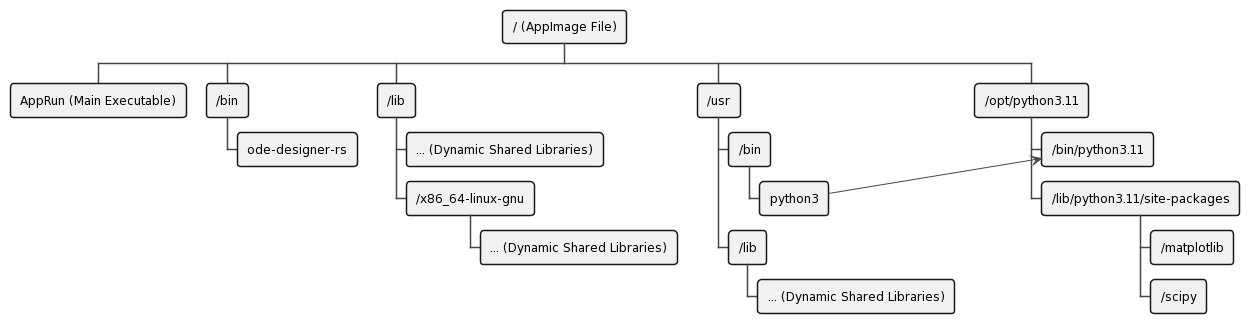
\includegraphics[scale=0.37]{diagrams/img/appimage.png} 
    \caption{Estrutura de diretórios da AppImage do software.}
    \label{fig:appimage}
\end{figure}

A AppImage contém a maioria das dependências de bibliotecas dinâmicas e inclui o interpretador de Python com as dependências necessárias pré-instaladas. Exceções às bibliotecas dinâmicas inclusas são as relacionadas às bibliotecas padrões de C e C++, que não devem ser 
distribuídas em versões mais novas. Como estas bibliotecas mantém retro-compatibilidade em novas versões, o software deve ser compilado numa distribuição com a menor versão suportada, garantindo funcionamento com versões mais novas.

Com o intuito de realizar este processo automaticamente, uma esteira de lançamento de versões foi desenvolvida. Ela se encarrega de compilar o software em um contêiner de Docker \cite{merkel2014docker} com uma versão de 2021 do sistema Debian com todas as dependências necessárias para fazer o software funcionar em sistemas Linux e Windows. 

\chapter{Aplicação do software na modelagem computacional}
\label{chap:resultados}
%Mostrar exemplos de modelos construídos e simulados com a ferramenta 

\section{Predador-presa}

O modelo predador-presa foi descrito na Seção \ref{sec:edos}. A Figura \ref{fig:predador-presa} mostra o modelo construído no software e a Figura \ref{fig:resultado-predador-presa} mostra um exemplo de resultado da simulação. 

\begin{figure}[h]
    \centering
    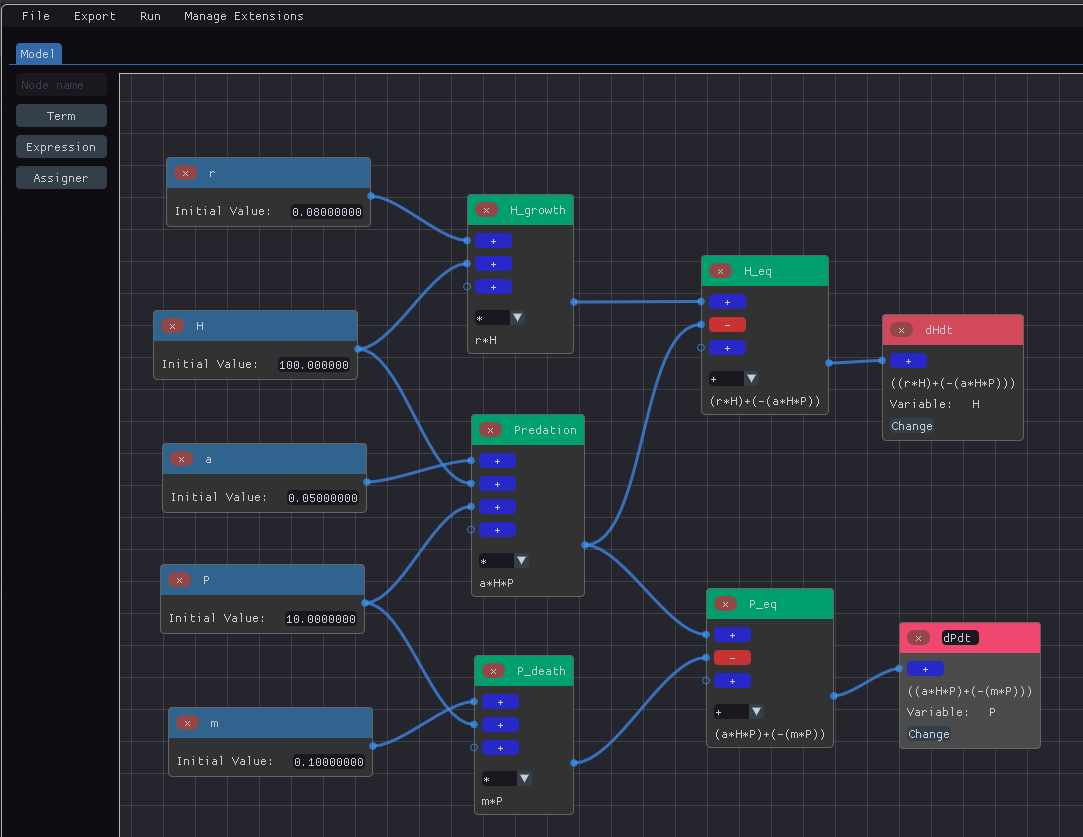
\includegraphics[width=\textwidth]{imgs/modelos/predador-presa.png} 
    \caption{Modelo predador-presa construído no software.}
    \label{fig:predador-presa}
\end{figure}

\begin{figure}[h]
    \centering
    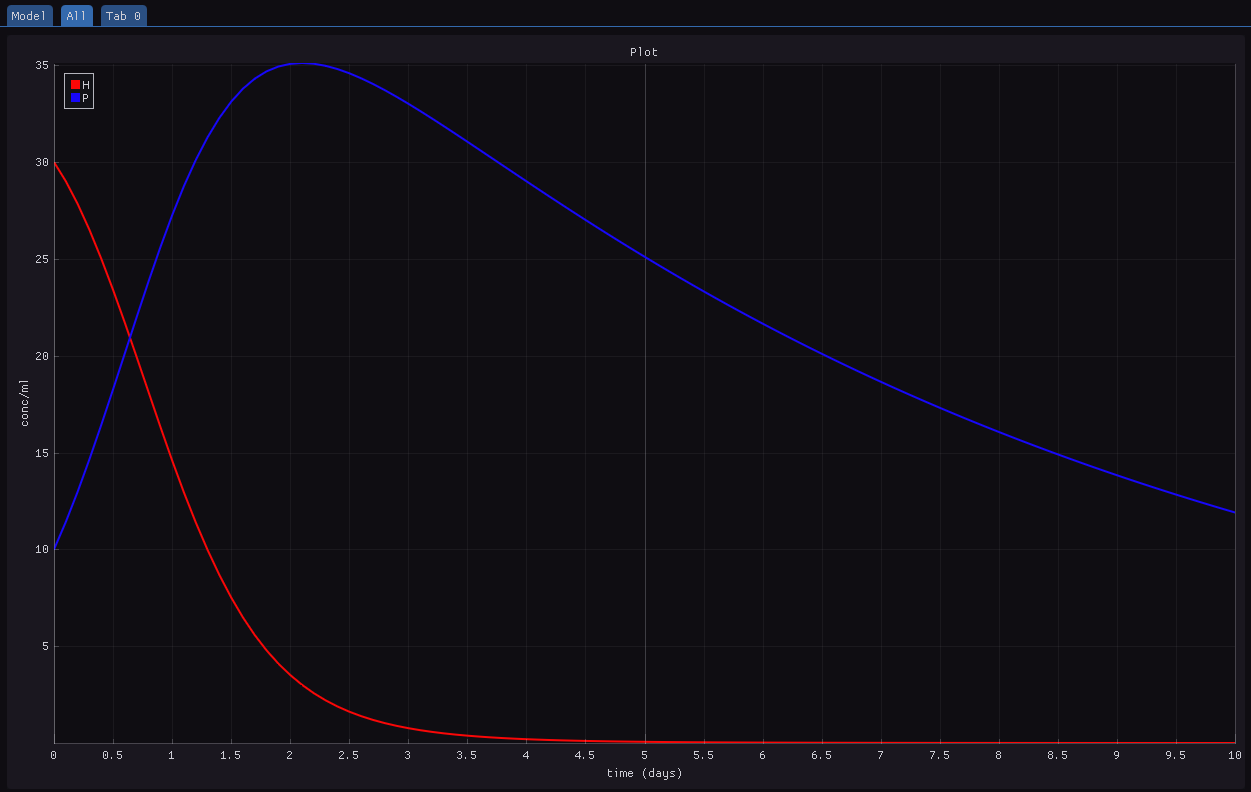
\includegraphics[width=\textwidth]{imgs/modelos/resultado-predador-presa.png} 
    \caption{Exemplo de resultado da simulação do modelo predador-presa.}
    \label{fig:resultado-predador-presa}
\end{figure}


\section{Transmissão de doenças}
%modelo SIRS 
Existem alguns modelos de EDOs clássicos para modelar a transmissão de um vírus na população como, por exemplo, modelo SIR, SIRS e SIS. Para mostrar a aplicação do software, foi construído o modelo SIRS que é composto pelo seguinte conjunto de EDOs: 

\begin{equation}\label{eq:sirs}
    \begin{array}{lr}
    \frac{dS}{dt} = -\beta.S.I + \gamma.R
    \\
    \\
    \frac{dI}{dt} = \beta.S.I - \alpha.I
    \\
    \\ 
    \frac{dR}{dt} = \alpha.I - \gamma.R
    \end{array}
\end{equation}

O modelo divide a população em indivíduos suscetíveis ($S$) à doença, infectados ($I$) e recuperados ($R$). Uma parte da população de suscetíveis pode se infectar (termo $\beta.S.I$). Os indivíduos infectados podem se recuperar com uma determinada probabilidade (termo $\alpha.I$) e os indivíduos recuperados podem voltar a ser suscetíveis à doença (termo $\gamma.R$).  

Na Figura \ref{fig:sirs}, podemos ver o modelo SIRS no software e na Figura \ref{fig:resultado-sirs} um exemplo de resultado da simulação do modelo. 

\begin{figure}[h]
    \centering
    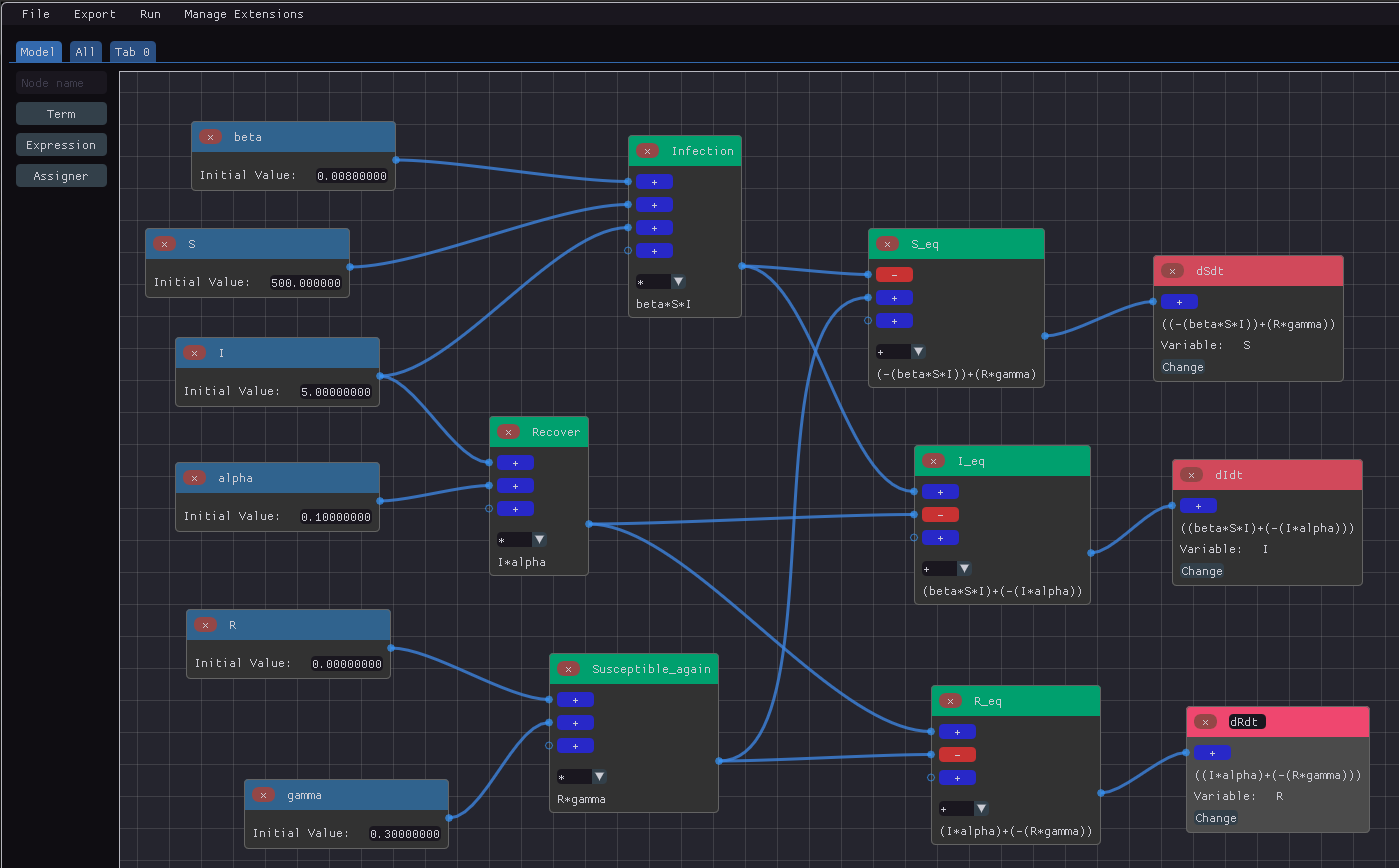
\includegraphics[width=\textwidth]{imgs/modelos/sirs.png} 
    \caption{Modelo SIRS construído no software.}
    \label{fig:sirs}
\end{figure}

\begin{figure}[h]
    \centering
    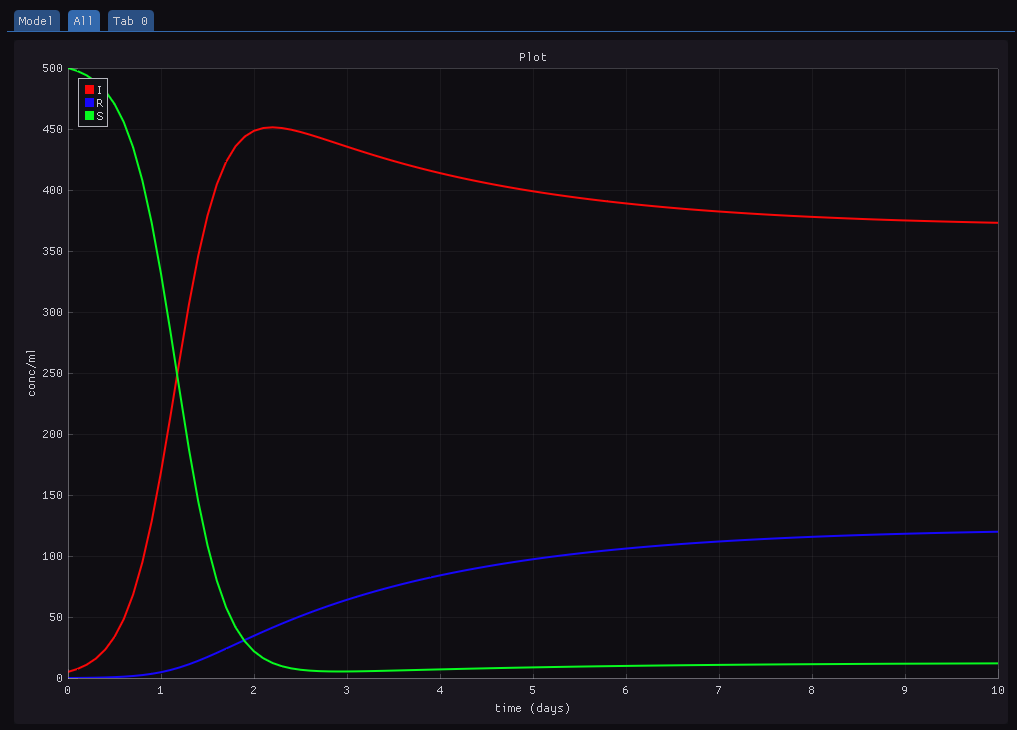
\includegraphics[width=\textwidth]{imgs/modelos/resultado-sirs.png} 
    \caption{Exemplo de resultado da simulação do modelo SIRS.}
    \label{fig:resultado-sirs}
\end{figure}

\section{Reação enzimática}

O modelo da reação enzimática com inibição competitiva modela uma reação química entre um substrato $S$ e uma enzima $E$ para formar um produto $P$. A enzima atua catalisando a reação e formando um complexo temporário $ES$ que pode voltar a se transformar em $E + S$ ou virar $E + P$. Essa reação é inibida por uma substância $I$ que se liga ao mesmo sítio de ligação do substrato $S$ na enzima $E$ formando um outro complexo chamado $EI$. Essa ligação impede a ligação de $S$ com $E$. O complexo $EI$ também tem um tempo de vida
finito e pode voltar a ser $E + I$.  
%(Referência: Mathematical modeling for enzyme inhibitors with slow and fast subsystems).
O sistema de EDOs que modela essa reação é dado na Equação \ref{eq:reacao}.

\begin{equation}\label{eq:reacao}
    \begin{array}{lr}
        \frac{dS}{dt} = k_2.ES - k_1.S.E 
        \\
        \\
        \frac{dP}{dt} = k_3.ES
        \\
        \\ 
        \frac{dI}{dt} = k_5.EI - k_4.E.I
        \\
        \\ 
        \frac{dES}{dt} = -k_2.ES + k_1.S.E - k_3.ES
        \\
        \\ 
        \frac{dEI}{dt} = -k_5.EI + k_4.E.I
        \\
        \\ 
        \frac{dE}{dt} = k_2.ES + k_3.ES + k_5.EI - k_1.S.E - k_4.E.I
    \end{array}
\end{equation}

A Figura \ref{fig:reacaoenzimatica} mostra o modelo da reação enzimática construído no software. 

\begin{figure}[h]
    \centering
    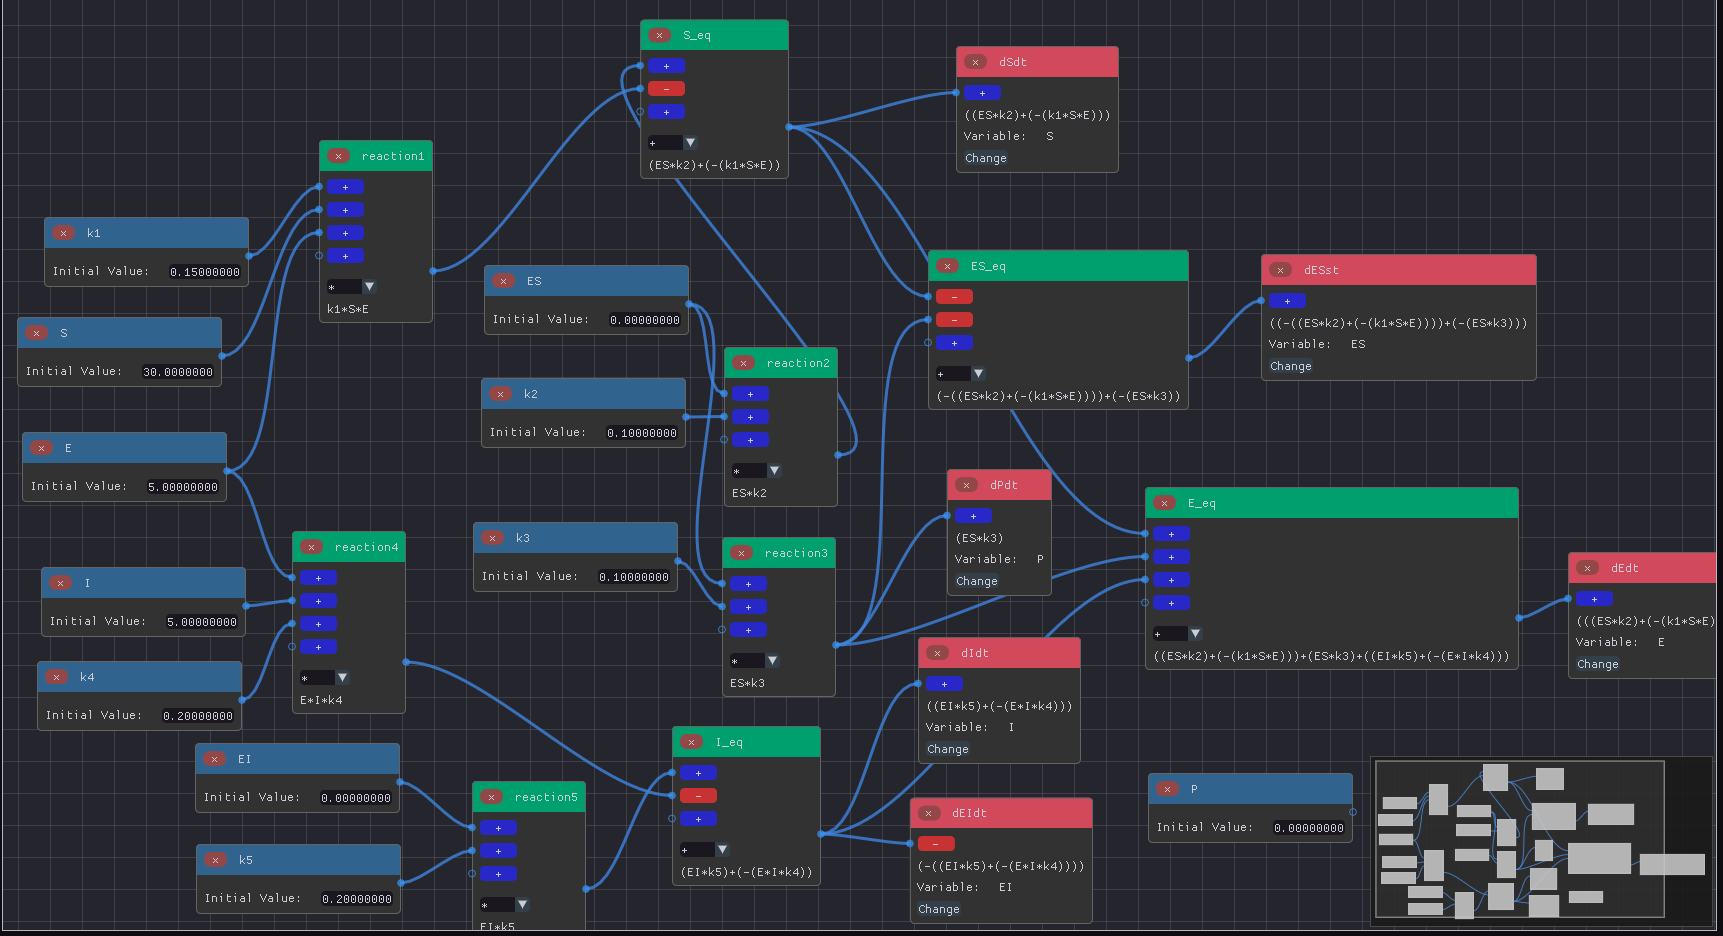
\includegraphics[width=\textwidth]{imgs/modelos/reacaoenzimatica.png} 
    \caption{Modelo da reação enzimática construído no software.}
    \label{fig:reacaoenzimatica}
\end{figure}
    
\section{Resposta imune a uma infecção viral}

O modelo apresentado nesta seção modela a resposta imune das células T a uma infecção viral. O modelo é descrito a seguir.  

As células epiteliais saudáveis ($E$) são infectadas pelo vírus ($V$) tornando-se infectadas ($I$) e também podem morrer devido ao dano ($D$) causado pelo resposta imune, isto é, devido ao dano mediado pelas células T efetoras ($T$). As células infectadas são eliminadas pelas células T ou podem morrer devido a ação dos vírus intracelulares. Com a morte da célula infectada, são liberados novos vírus no tecido. Os vírus são eliminados pela ação dos anticorpos e outras células de defesa que não são explicitamente representadas no modelo. As células T migram para o tecido devido a ação das citocinas pró-inflamatórias ($C$). Esse processo foi simplificado porque não considera-se, no modelo atual, as células T \textit{helper} e outros níveis de ativação das células T de forma explícita. As citocinas pró-inflamatórias são produzidas pelas células T na presença de marcadores inflamatórios da infecção.   

\begin{equation}
    \begin{array}{lr}
        \frac{dD}{dt} = \beta.(T + 2.I) - m_D.D
        \\
        \\
        \frac{dE}{dt} = - k_E.E.V 
        \\
        \\
        \frac{dI}{dt} = k_E.E.V - k_I.I.T - a.I
        \\
        \\
        \frac{dV}{dt} = a.I - k_V.V
        \\
        \\
        \frac{dT}{dt} = s_T.(1+C)  - m_T.T
        \\
        \\
        \frac{dC}{dt} = beta_C.T.(I + V) – m_C.C
    \end{array}
\end{equation}

Na Figura \ref{fig:infeccaoviral}, é apresentada parte do modelo construído no software.

\begin{figure}[h]
    \centering
    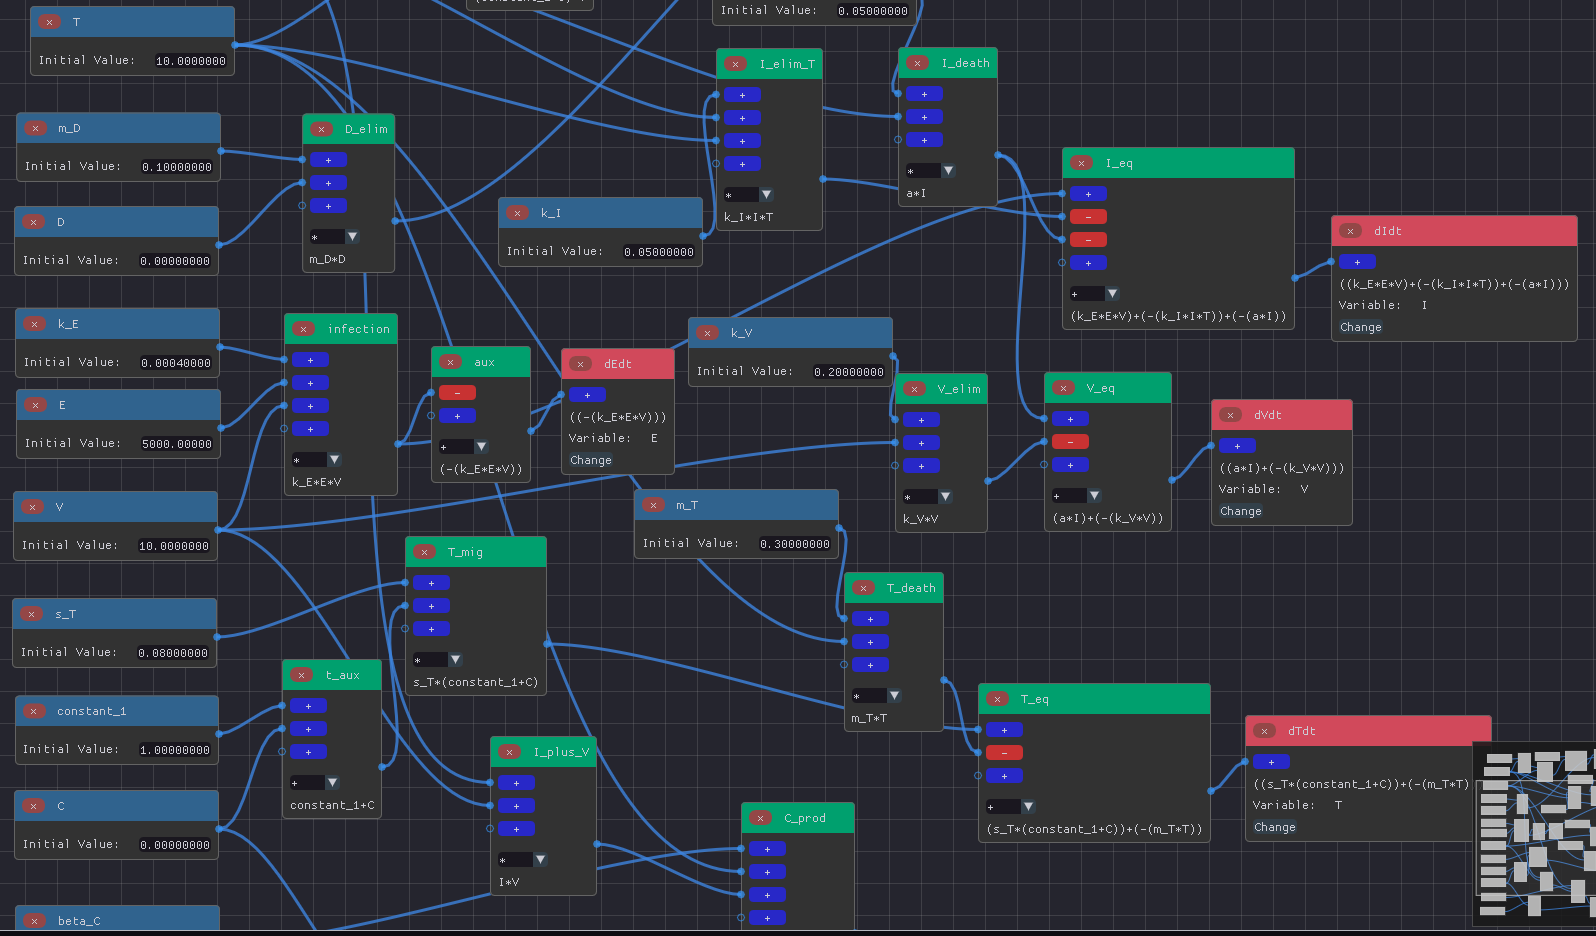
\includegraphics[width=\textwidth]{imgs/modelos/infeccaoviral.png} 
    \caption{Modelo da infecção viral construído no software.}
    \label{fig:infeccaoviral}
\end{figure}

%-----------------------------//----------------------------
\chapter{Conclusão e trabalhos futuros}
\label{chap:conclusao}

%TODO: conclusões
Neste trabalho, foi desenvolvido um software para automatizar a criação e simulação de modelos computacionais baseados em EDOs. ... 

Destaca-se as seguintes possibilidades de trabalhos futuros: 
\begin{itemize}
    \item Geração do código do modelo em Rust e simulação das EDOs em "tempo real";
    \item Simulação de modelos estocásticos com o algoritmo de Gillespie utilizando o mesmo editor baseado em nós, fornecendo como outra opção de exportação; 
    \item Suporte a ajuste de parâmetros fornecendo recursos para carregamento dos dados experimentais, escolha das variáveis e parâmetros a serem ajustados e plotagem dos gráficos e dos dados experimentais após a execução do ajuste; 
    \item Adição de recursos para a análise de sensibilidade de parâmetros;
    \item Criação e implementação de uma representação baseada em grafos para uma visualização mais alto nível das interações do modelo. O foco será na visualização de modelos do sistema imune; 
    \item Adição de novos nós como, por exemplo, nós para difusão, quimiotaxia, para dar suporte a criação de modelos de Equações Diferenciais Parciais (EDPs). Implementação da geração de código para as EDPs utilizando o método de diferenças finitas. Essa implementação exigiria uma mudança maior na interface e na representação intermediária para acomodar características e recursos que são próprios de modelos de EDPs; 
    \item Desenvolvimento de uma versão Web do software para que ele possa ser utilizado por um número maior de pessoas. A criação do modelo será feita através do navegador Web e todo o processamento incluindo a geração de código, execução, geração dos resultados e imagens será feita no servidor. As tecnologias usadas pelo projeto até então são todas compatíveis com a Web. A linguagem Rust, baseada na LLVM, possui suporte nativo à WebAssembly.
\end{itemize}

%TODO: Falar das limitações do trabalho 
Como limitações do software, destaca-se que atualmente é difícil criar modelos muito complexos porque dependendo da quantidade de nós e ligações do modelo, fica difícil entender como cada parte do modelo é combinada para formar as EDOs, sendo uma limitação da representação visual.  

%Solução: Uma ideia é oferecer a possibilidade de agrupar um grupo de nós e as ligações entre eles em um submodelo. Os submodelos seriam combinados para formar o modelo completo. 

% % ---
% % Finaliza a parte no bookmark do PDF, para que se inicie o bookmark na raiz
% % ---
% \bookmarksetup{startatroot}% 
% % ---

% % ---------------------------------------------------------------------------------------------
% % ---------------------------------------------------------------------------------------------
% % ----------------------------------------------------------------------ELEMENTOS PÓS-TEXTUAIS-
% % ---------------------------------------------------------------------------------------------
% % ---------------------------------------------------------------------------------------------
\postextual

% % ----------------------------------------------------------
% % Referências bibliográficas
% % ----------------------------------------------------------
\bibliographystyle{abntex2-alf}
\bibliography{referencias}

% % ---------------------------------------------------------------------------------------------
% % ------------------------------------------------------Apêndices - Caso não existam, comentar-
% % ---------------------------------------------------------------------------------------------
%\begin{apendicesenv}
	
	% Imprime uma página indicando o início dos apêndices
	\partapendices


\end{apendicesenv}

\appendix {

\section{Código de Python gerado para o modelo Predador-Presa}
\label{code:predador-presa}
Código completo \attachfile{code/dhdp.py}
\lstinputlisting[language=Python]{code/dhdp-part.py}

\section{RI do modelo Predador-Presa}
\label{ri:predador-presa}
Arquivo JSON \attachfile{code/dhdp.json}

}

% % ---------------------------------------------------------------------------------------------
% % ---------------------------------------------------------Anexos - Caso não existam, comentar-
% % ---------------------------------------------------------------------------------------------
% %% ---
% Inicia os anexos
% ---
\begin{anexosenv}

% Imprime uma página indicando o início dos anexos
\partanexos

% ---
\chapter{Morbi ultrices rutrum lorem.}
% ---

Lorem ipsum dolor sit amet, consectetur adipiscing elit. Maecenas laoreet porttitor dui sit amet tempus. Phasellus finibus ac tortor eget lobortis. Suspendisse et nunc velit. Vestibulum vulputate, urna laoreet hendrerit dignissim, urna massa facilisis ante, quis vestibulum erat elit blandit eros. Cras a justo eu risus lobortis lobortis vitae luctus mauris. Nunc congue consequat justo, eget imperdiet magna porttitor nec. Class aptent taciti sociosqu ad litora torquent per conubia nostra, per inceptos himenaeos. Vestibulum lorem ex, vulputate nec nibh ac, consequat vulputate ex. Aliquam dignissim dapibus orci, eget porttitor dui rutrum a. Pellentesque lacinia ante in sapien lacinia, a ultrices libero faucibus. In erat purus, elementum ut lectus nec, iaculis accumsan mi. Donec bibendum ante ac nulla hendrerit consectetur. Aliquam a mauris ultricies, ornare lacus sed, convallis orci. Class aptent taciti sociosqu ad litora torquent per conubia nostra, per inceptos himenaeos.

Etiam viverra risus non sodales vehicula. In convallis sapien vel neque aliquam, non porttitor turpis dapibus. Suspendisse consectetur volutpat purus, quis ultrices odio tempor id. Duis laoreet justo quam, vitae ultrices tellus dapibus vel. Mauris placerat ipsum finibus odio luctus suscipit. Duis facilisis non leo non varius. Sed et magna feugiat, rutrum diam vel, maximus nunc.

% ---
\chapter{Cras non urna sed feugiat cum sociis natoque penatibus et magnis dis
parturient montes nascetur ridiculus mus}
% ---


Lorem ipsum dolor sit amet, consectetur adipiscing elit. Maecenas laoreet porttitor dui sit amet tempus. Phasellus finibus ac tortor eget lobortis. Suspendisse et nunc velit. Vestibulum vulputate, urna laoreet hendrerit dignissim, urna massa facilisis ante, quis vestibulum erat elit blandit eros. Cras a justo eu risus lobortis lobortis vitae luctus mauris. Nunc congue consequat justo, eget imperdiet magna porttitor nec. Class aptent taciti sociosqu ad litora torquent per conubia nostra, per inceptos himenaeos. Vestibulum lorem ex, vulputate nec nibh ac, consequat vulputate ex. Aliquam dignissim dapibus orci, eget porttitor dui rutrum a. Pellentesque lacinia ante in sapien lacinia, a ultrices libero faucibus. In erat purus, elementum ut lectus nec, iaculis accumsan mi. Donec bibendum ante ac nulla hendrerit consectetur. Aliquam a mauris ultricies, ornare lacus sed, convallis orci. Class aptent taciti sociosqu ad litora torquent per conubia nostra, per inceptos himenaeos.

Etiam viverra risus non sodales vehicula. In convallis sapien vel neque aliquam, non porttitor turpis dapibus. Suspendisse consectetur volutpat purus, quis ultrices odio tempor id. Duis laoreet justo quam, vitae ultrices tellus dapibus vel. Mauris placerat ipsum finibus odio luctus suscipit. Duis facilisis non leo non varius. Sed et magna feugiat, rutrum diam vel, maximus nunc.

Donec vehicula dapibus pharetra. Etiam et libero pharetra nulla ultricies laoreet sit amet vel sapien. Proin ultrices vitae nibh quis accumsan. Nullam in tortor erat. Quisque imperdiet dui venenatis pulvinar laoreet. Nulla ut nunc sed urna consectetur finibus id ut justo. Sed in placerat massa, quis tempor orci.


\end{anexosenv}

% %---------------------------------------------------------------------
% % INDICE REMISSIVO
% %---------------------------------------------------------------------
% %\printindex

\end{document}
